% Nejprve uvedeme tridu dokumentu s volbami
\documentclass[czech,master]{diploma}
% Dalsi doplnujici baliky maker
\usepackage[autostyle=true,czech=quotes]{csquotes} % korektni sazba uvozovek, podpora pro balik biblatex
\usepackage[backend=biber, style=iso-numeric, alldates=iso]{biblatex} % bibliografie

%\usepackage{biblatex}
\usepackage{dcolumn} % sloupce tabulky s ciselnymi hodnotami
\usepackage{subfig} % makra pro "podobrazky" a "podtabulky"
\usepackage[cpp]{diplomalst}
\usepackage{lscape}
\usepackage{longtable}
\usepackage{xcolor}



% Zadame pozadovane vstupy pro generovani titulnich stran.
\ThesisAuthor{Marek Bauer}

\ThesisSupervisor{Ing. Jan Kožusznik, Ph.D.}

\CzechThesisTitle{Nástroj pro tvorbu FMEA analýzy}

\EnglishThesisTitle{Tool for FMEA Analysis}

\SubmissionYear{2022}

\ThesisAssignmentFileName{ThesisSpecification_BAU0027.pdf}

% Pokud nechceme nikomu dekovat makro zapoznamkujeme.
\Acknowledgement{Rád bych na tomto místě poděkoval všem, kteří mě podporovali při tvorbě této práce. Konkrétně mému vedoucímu Ing. Janu Kožusznikovi, Ph.D. za konzultace, pracovníkům studovny za poskytnutí prostoru k práci a mým dvěma kamarádům Janu Bauerovi a Františkovi Šumšalovi za provedení testovacích případů.}

\CzechAbstract{Tato diplomová práce se zabývá problematikou správy rizik v rámci různých fází při vývoji a výrobě nových produktů.  Konkrétně práce cílí na metodu FMEA zaměřenou na odhalení a mitigaci rizik \linebreak v rámci návrhu produktu a následného výrobního procesu. Tato metoda se narozdíl od jiných provádí před samotnou výrobou produktu ve snaze předcházet možným rizikům. V rámci této diplomové práce také vznikl nástroj, který umožňuje vypracování metody FMEA. Hlavními rysy nástroje jsou možnost souběžné práce týmu provádějící analýzu a přehledný grafický a textový režim sloužící pro náhled i tvorbu v rámci jednotlivých kroků analýzy. Dále nástroj nabízí další podpůrné funkce jako je nastavení vlastních kritérií hodnotících atributů, kontrola úplnosti analýzy, tvorba zápisů \linebreak ze setkání, import a export analýzy. }

\CzechKeywords{FMEA, návrh, výrobní proces, způsoby selhání, příčiny selhání, důsledky selhání, webová aplikace}

\EnglishAbstract{This diploma thesis deals with the issue of risk management within the various phases of the development and production of new products. Specifically, the thesis aims at the FMEA method targeted at detecting and mitigating risks within the product design and subsequent production process. This method, unlike the others, is performed before the actual production of the product in an attempt to prevent possible risks. As part of this thesis, a tool was also created that enables the development of the FMEA method. The main features of the tool are the possibility of simultaneous work of the team performing the analysis and a clear graphic and text mode used for preview and creation within the individual steps of the analysis. Furthermore, the tool offers other supporting functions such as setting your own criteria for evaluating attributes, checking the completeness of the analysis, creating meeting loggs, importing and exporting the analysis.}

\EnglishKeywords{FMEA, design, manufactoring process, failure modes, failure causes, failure effects, web application}

\AddAcronym{FMEA}{Failure Mode and Effect Analysis}
\AddAcronym{DFMEA}{Design Failure Mode and Effect Analysis}
\AddAcronym{PFMEA}{Process Failure Mode and Effect Analysis}
\AddAcronym{AIAG}{Automotive Industry Action Group}
\AddAcronym{VDA}{Verband der Automobilindustrie}
\AddAcronym{RPN}{Risk Priority Number}
\AddAcronym{AP}{Action Priority}
\AddAcronym{PPAP}{Production Part Approval Process}
\AddAcronym{SPC}{Statistical Process Controll}
\AddAcronym{MSA}{Measurement System Analysis}
\AddAcronym{4M}{Machine, Man, Material, Milieu}
\AddAcronym{FMEA-MSR}{Failure Mode and Effect Analysis - Monitoring and System response}
\AddAcronym{UI}{User Interface}
\AddAcronym{FMECA}{Failure Modes, Effects and Criticality Analysis}
\AddAcronym{RPFMEA}{Failure Mode and Effect Analysis}
\AddAcronym{}{}
\AddAcronym{}{}
\AddAcronym{}{}
\AddAcronym{}{}
\AddAcronym{}{}
\AddAcronym{}{}
\AddAcronym{}{}
\AddAcronym{}{}
\AddAcronym{}{}
\AddAcronym{}{}
\AddAcronym{}{}
\AddAcronym{}{}
\AddAcronym{}{}
\AddAcronym{}{}
\AddAcronym{}{}
\AddAcronym{}{}




\addbibresource{literature.bib}
%\addbibresource{coffee.bib}

% Novy druh tabulkoveho sloupce, ve kterem jsou cisla zarovnana podle desetinne carky
\newcolumntype{d}[1]{D{,}{,}{#1}}


% Zacatek dokumentu
\begin{document}

% Nechame vysazet titulni strany.
\MakeTitlePages

% Jsou v praci obrazky? Pokud ano vysazime jejich seznam a odstrankujeme.
% Pokud ne smazeme nasledujici dve makra.
\listoffigures
\clearpage

% Jsou v praci tabulky? Pokud ano vysazime jejich seznam a odstrankujeme.
% Pokud ne smazeme nasledujici dve makra.
\listoftables
\clearpage

% A nasleduje text zaverecne prace.
\chapter{Úvod}
\label{sec:Uvod}
V mnoha odvětvích lidské činnosti je možné přijít do styku s nedokonalostmi v návrzích produktů nebo výrobních procesech, které mohou vést k nezamýšlenému chování a více či méně važným následkům. Následky mohou být triviální, které výrazným způsobem neomezují funkci produktu nebo naopak vážné, které mohou být životu nebezpečné. Dalším důsledkem špatného technologického procesu nebo návrhu je samozřejmě také finanční stránka, kdy nadměrná produkce disfunkčních dílů stojí výrobce peníze navíc za materiál nebo při objevení závady až u koncové zákazníka také výdaje s vyřizováním reklamací, opravami a podobně. Tyto důvody vedly k vytvoření procesů, metod a norem, které mají za cíl odhalení, odstranění nebo alespoň zmírnění možných závad a rizik ještě před začátkem realizace dané činnosti. Souhrně lze tyto snahy označit Risk Management, tedy disciplínu zabývající se správou a řízením rizik. 

Jednou z těchto metod je analytická metoda FMEA(Failure Mode and Effects Analysis), kterou se zabývá tato diplomová práce. Následující kapitola  \ref{sec:FMEA} bude obsahovat základní popis této metody spolu s její historií, dále popis v jakých oborech se metoda aktuálně nejvíce uplatňuje a také rozdělení na základní typy podle toho v jaké fázi vývoje produktu se analýza provádí.

Kapitola \ref{sec:FMEA_postup} se budou zabývat tím, jaký je postup při vypracovávání této analýzy. Analýza se skládá celkem ze sedmi kroků, které budou podrobně vysvětleny. Budou zde také uvedeny výňatky tabulky z formulářů, ve kterých se analýza provádí. Na jednotlivých krocích analýzy budou zobrazeny odlišnosti dvou typů analýz, na které je práce zaměřena.

Následovat bude kapitola \ref{sec:pozadavky} sloužící jako popis požadavků na vytvářený nástroj. Specifikace požadavků bude inspirována disciplínou inženýrství požadavků. Požadavky budou členěny dle typů a kapitol, budou obsahovat popis a také jejich konečný stav, podle toho jak se vyvýjel v rámci průběhu návrhu a implementace. Některé zajímavé požadavky budou popsány detailněji z důvodu vysvětlení důvodu jejich zařazení nebo naopak nezařazení do celkové sady požadavků na vyvýjený nástroj. Tento seznam požadavků vychází jak ze samotného zadaní diplomové práce, tak z konzultací s vedoucím práce a také rešerše existujících řešení, kterou se bude zabývat kapitola \ref{sec:nastroje}. 

Rešerše existujících řešení je cíleně umístěna až za kapitolou zabývající se analýzou a specifikací požadavků z toho důvodu, že budou v této kapitole srovnány jednotlivé nástroje na základě zjednodušené sady požadavků vzniklé v předchozí kapitole. Součástí srovnání bude i nástroj vytvořený autorem této práce, kde bude vidět srovnání, jak byly jednotlivé požadavky naplněny oproti profesionálním řešením. 

Další kapitola číslo \ref{sec:navrh} se již bude zabývat vlastním nástrojem, který byl vytvořen v rámci této diplomové práce. Bude obsahovat popis architektury, použitých technologií, návrh databáze a uživatelského rozhraní. Budou zde uvedeny i důvody proč byly jednotlivé návrhové rozhodnutí učiněny. 

Popisem implementace vytvořeného nástroje se bude zabývat kapitola \ref{sec:implementace}. Implementace bude rozdělena na klientskou a serverovou část. Popis bude brán jak z uživatelského, tak implementačního hlediska. Budou zde podrobněji ukázány jednotlivé vlastnosti a funkce nástroje. Konec kapitoly se bude zabývat testováním vytvořeného nástroje ve formě integračních testů. 

Závěrem bude hodnocení dosažených výsledků a vytvořeného nástroje. Budou zde také uvedeny různé možnosti rozšíření nástroje, které z různých důvodu nebyly implementovány. 
\endinput
\chapter{FMEA}
\label{sec:FMEA}
FMEA je zkratka z anglického výrazu Failure Mode and Effect Analysis, česky lze toto označení přeložit jako Analýza výskytu vad a jejich dopadů nebo Analýza příčin a důsledků. Jedná se tedy o analytickou metodu, která ma za cíl odhalení možných vad ve výrobním procesu nebo návrhu produktu, nalezení příčin výskytu těchto vad, ohodnocení závažnosti daného rizika a snaha o jeho zmírnění nebo odstranění. Na vypracování této analýzy se většinou podílí tým odborníků z různých oblastí daného odvětví, kteří využají svých znalostí a zkušeností ze svých profesí k odbornému posouzení problémů v různých fázích analýzy. Obvykle tento tým tvoří vedoucí výroby, zástupce z oddělení pro kontrolu kvality, konstruktér, technolog popřípadě další odborníci. Mezi relevantní účastníky také může patřit zákazník, kterému mohou být poskytovány výstupy z jednotlivých verzí analýzy. V tomto případě může být FMEA součástí smluvní dohody mezi výrobcem a zákazníkem jako záruka kvality například v rámci PPAP (Production Part Approval Process). Přesto, že je FMEA prováděna před začátkem realizace dané fáze vývoje, je dobré přistupovat k dokumentům obsahujícím analýzu jako k dynamickým a v čase zlepšovat jejich kvalitu a přesnost.  

\section{Historie FMEA}
\label{sec:historie}
Počátky FMEA sahají do 40. let minulého století, kdy byla FMEA poprvé použita americkou armádou pro redukci potenciálních závad při výrobě munice. Metoda se ukázala jako vysoce efektivní a kolem roku 1960 ji začlenila do svých přípravných technik i společnost NASA. FMEA se ukázala jako podstatná součást mise Apollo. Od 70.let 20. století již následoval automobilový průmysl, který tvoří jedno z hlavních odvětví, kde je tato metoda využívána. Prvotním uživatelem byla automobilka Ford, která přijala FMEA jako reakci na špatný bezpečnostní stav jejich modelu Ford Pinto. Jejich příkladu pak následovali další američtí i evropští výrobci. Tyto události vedly ke vzniku asociací AIAG a VDA, které definují standardy pro zvýšení kvality pomocí nástrojů jako je FMEA, SPC(statistical process controll) nebo MSA(Measurement system analysis). Z důvodu rozšířenosti použití FMEA analýzy v tomto průmyslu bude i v následujících popisech a příkladech brán pohled na tvorbu FMEA z toho odvětví.  

\section{Aplikace FMEA}

FMEA se člení zejména na tři typy, které se odvíjejí podle fáze vývoje. Jedná se o tyto tři druhy: 

\begin{itemize}
	\item  DFMEA (Design)
	\item  PFMEA (Process)
	\item  SFMEA (System)
\end{itemize}
V této diplomové práci bude věnována pozornost hlavně analýze zaměřené na návrh a proces. Tyto dvě zaměření jsou v praxi využívány nejvíce pravděpodobně díky tomu, že se zaměřují na specifičtější části vývoje produktu. Součástí FMEA analýzy je dekompozice subjektu ve fázi strukturální analýzy na nízkoúrovňové části, pro které se lépe hledájí možné způsoby selhání. Použití metody na celý systém se tak může zdát jako zbytečně komplexní řešení a v některých případech tato možnost ani nepřipadá v úvahu. Konkrétně je dobré uvést příklad z rozsáhlého autombilového průmyslu, kde se výroba vozu skládá ze spolupráce několika různých výrobců komponent, kteří často nemusí mít přehled o práci ostatních dodavatelů. V některých případech jsou výrobky součástí většího celku a těžko se při použití metody DFMEA nalézají všechny možné rizikové scénáře. V těchto případech se například provádí pouze analýza zaměřená na konkrétní výrobní proces(PFMEA), u kterého lze určit možná rizika. 

\subsection{DFMEA}
\label{subsec:DFMEA}
DFMEA se používá pro analýzu nových návrhu produktů. Měla by tedy navazovat na ukončení fáze návrhu a vycházet tak ze softwarových artefaktů z toho vyplývajících. Jedním z těchto artefaktů může být například blokový diagram(Boundary diagram), který pokrývá určitou část systému. Pomocí blokového diagramu lze zobrazit rozhraní a vztahy mezi jednolivými komponentami. Mezi další podklady pro tvorbu DFMEA může patřit: 
\begin{itemize}
	\item  Normy a předpisy
	\item  Fyzikální specifikace materiálů
	\item  Návrhy obdobných produktů, popř. DFMEA pokud byla provedena
	\item  Požadavky zákazníka
	\item  Diagram parametrů (P-diagram)
	\item  Shrnutí všech požadavků na návrh
	
\end{itemize}

Stejně jako u ostatních typů FMEA je i zde potřeba průběžně aktualizovat softwarové artefakty i při přechodu do dalších fází vývoje produktu. Postup pro vypracovaní DFMEA by se dal rámcově shrnout do těchto bodů: 
\begin{enumerate}
	\item Identifikace rizik
	\item Analýza rizik
	\item Hodnocení a řízení rizik 
	\item Návrh optimalizačních opatření
	\item Přehodnocení rizik
\end{enumerate}
Podprobnějším popisem struktury a kroků, které se provádí při vypracování DFMEA se bude zabývat kapitola \ref{sec:FMEA_postup}

\subsection{PFMEA}
\label{subsec:PFMEA}
PFMEA se používá pro analýzu nových procesů zejména z pohledu výroby. Dá se říci, že by měla navazovat ne předchozí analýzu návrhu produktu, kdy výrobní proces je dalším logickým krokem při vývoji. Mezi další vstupní předpoklady patří například flow diagram, který dekomponuje proces do série nazujících kroků. V praxi je možné setkat se i s případem, kdy se PFMEA provádí až jako snaha o zlepšení stávajícího procesu. V tomto případě lze jako podklad pro vypracování také vzít v úvahu fyzickou prohlídku výrobní haly. Tuto analýzu často vykonává stejný tým jako v případě DFMEA.  



\endinput
\chapter{Vypracování FMEA }
\label{sec:FMEA_postup}
V této kapitole bude podrobněji popsán postup při použití metody FMEA pro návrh a proces. Obě tyto varianty mají totožnou strukturu a tak budou její jednotlivé části popsány zároveň pro vytvoření obrazu v jakých atributech se konkrétní části obou typů analýz liší. 

Výňatky z formulářů odpovídají standardu příručky FMEA pro automobilový průmysl\cite{fmeaHandbook} Jednotlivé reprezentace FMEA se mohou lišit, zejména při použití v odlišných odvětvích. Jak již bylo naznačeno v kapitole \ref{sec:historie}, tak lze analýzu aplikovat v odvětvích jako je armádní průmysl, zdravotnictví, kosmický průmysl a mnoho dalších. Nicméně nejrozšířenějším odvětvím, který využívá metody FMEA, je automobilový průmysl a i proto budou uvedené příklady z tohoto odvětví. Také je možné se setkat s některými volitelnými atributy, které nemají veliký význam a nebude na ně brán v následujícím popisu zřetel.  

\section{Plánování a příprava(1. krok)}
V kapitolách \ref{subsec:DFMEA} a \ref{subsec:PFMEA}  byly zmíněny předpoklady a vstupní podmínky před začátkem samotné analýzy. V prvník kroku je také sestaven tým odborníků, kteří budou za pomocí společných setkání provádět samotnou analýzu. V týmu je potřeba před začátkem práce definovat základní pravidla a pojmy. Je potřeba definovat škálu pro atributy, pomocí kterých bude probíhat hodnocení nalezených rizik. Od této škály se například bude odvíjet, od jaké hodnoty bude akceptována určitá míra rizika. Tyto atributy jsou: 

\begin{enumerate}
	\item Severity (Význam)
	\item Occurance (Výskyt)
	\item Detection (Odhalitelnost)
\end{enumerate}

Pro každou z těchto tří atributů je potřeba stanovit škálu, která nabývá hodnot od jedné do desíti a každé hodnocení obsahuje slovní popis této hodnoty pro jednodušší určení hodnoty. 

Po stanovení těchto atributů je možné přistoupit k vyplnění úvodních informací tvořící hlavičku analýzy. 

\begin{center}
\begin{table}[h]
	\centering
	\caption{Hlavička analýzy}
 \label{tab:header_FMEA}
	\label{tab:Head1}
        \begin{tabular}{|c | r | l |} 
         \hline
 \multicolumn{3}{|c|}{Planning and preparation (Step 1)} \\

         \hline
         1 & Company Name & ABC  \\ [0.5ex] 
         \hline
         2 & Location & Bratislava  \\ [0.5ex] 
         \hline
         3 & Customer Name & VW Group  \\ [0.5ex] 
         \hline
         4 & Model Year / Program(s) & 2006/J77 \\ [0.5ex] 
         \hline
         5 & Subject & J77 Instrument Cluster \\ [0.5ex] 
         \hline
         6 & Responsibility & John Doe (Product Eng.) \\ [0.5ex] 
         \hline
         7 & D(P)FMEA Start Date & 1.1.2023  \\ [0.5ex] 
         \hline
         8 & D(P)FMEA Revision Date & 27.2.2023 \\ [0.5ex] 
         \hline
         9 & D(P)FMEA ID Number & 77 \\ [0.5ex] 
         \hline
         10 & Confidentiality Level & Proprietary \\ [0.5ex] 
         \hline
         11 & Cross-Functional team & John Doe, Henry Smith \\ [0.5ex] 
         \hline
        \end{tabular}
    \end{table}
\end{center}

Tabulka \ref{tab:header_FMEA} obsahuje seznam atributů, které se vyplňují v rámci úvodní fáze analýzy. Zde je popis jednotlivých atributů:

\begin{enumerate}
	\item \textbf{Název společnosti} - jedná se o společnosti v rámci, které je analýza prováděna
	\item \textbf{Lokace} - zde může lokace odpovídat buď lokací inženýrského týmu zodpovědného za návrh produktu(DFMEA) nebo umístěním výrobního závodu(PFMEA) 
	\item \textbf{Jméno zákazníka} - Podle zaměření analýzy, může být zákazníkem jak koncový uživatel, tak i interní oddělení, které navazuje ve výrobním cyklu
 \item \textbf{Modelový rok, Program} - specifikace modelu produktu, program(DFMEA) nebo platforma(PFMEA)
 \item \textbf{Předmět} - vysokoúroňový popis zkoumaného prvku
 \item \textbf{Zodpovědnost} - vlastník dokumentu analýzy, často v roli manažera setkání týmu
 \item \textbf{Začátek analýzy} - počáteční datum
 \item \textbf{Datum revize} - datum kontroly provedených změn 
 \item \textbf{Identifikační číslo analýzy} - jedná se o interní hodnotu, má smysl v rámci kontextu firmy, kdy může sloužit jako odkaz na dokument s analýzou
 \item \textbf{Stupeň důvěrnosti} - může nabývat hodnot (obchodní, proprietární, důvěrný)
 \item \textbf{Multioborový tým} - seznam lidi podílejících se na tvorbě analýzy
\end{enumerate}

\section{Analýza struktury(2. krok)}
\label{sec:FMEA_postup_2}
Cílem strukturální analýzy je dekompozice zkoumaného produktu nebo procesu na menší části, které pak slouží jako vstupní parametry v dalších krocích. Dekompozice slouží pro jednodušší pochopení zkoumaného produktu. Výsledkem je nejčastěji stromová struktura o výšce stromu tři, kdy kořenem stromu je přímo zkoumaný prvek.





\begin{center}
\begin{table}[h]
	\centering
	\caption{Formulář pro analýzu struktury(DFMEA) }
	\label{tab:structure_DFMEA}
\begin{tabular}{ |p{4cm}|p{3cm}|p{3cm}|  }
 \hline
 \multicolumn{3}{|c|}{Structure Analysis (Step 2)} \\
 \hline
 1. Next Higher Level& 2.Focus Element
No. And Name of Focus Element &3. Next Lower Level of Characteristic Type\\
 \hline
 Instrument Cluster B90   & 6. Speed clock    &Stepper motor\\


 \hline
\end{tabular}\  
\end{table}
\end{center}

\begin{center}
\begin{table}[h]
	\centering
	\caption{Formulář pro analýzu struktury(PFMEA) }
	\label{tab:structure_PFMEA}
\begin{tabular}{ |p{4cm}|p{3cm}|p{3cm}|  }
 \hline
 \multicolumn{3}{|c|}{Structure Analysis (Step 2)} \\
 \hline
1. Process Item
System, Subsystem, Part Element or Name of Process
& 2. Process Step
No. And Name of Focus Element
&3. Process Work Element

4M Type\\
 \hline
X98 sun roll assembly line   & 020 Assembly body-mechanism   &Operator\\


 \hline
\end{tabular}\  
\end{table}
\end{center}

V tomto kroku analýzy se nejvíce projevují rozdíly mezi jejími dvěma zmíněnými typy. Rozdílnost atributů, které jsou v této fázi vyplňovány je možné porovnat v tabulkách \ref{tab:structure_DFMEA} a  \ref{tab:structure_PFMEA} 
Dále následuje popis jednotlivých atributů, které se vyplňují v rámci strukturální analýzy. 

\begin{enumerate}
	\item \textbf{Vyšší úroveň / Položka procesu systému, subsystému, dílu nebo název procesu} - Prvek na nejvýšší úrovni v rámci předmětu analýzy, pro tento prvek se v se v rámci analýzy selhání definují důsledky selhání
	\item \textbf{Vybraný prvek, číslo a označení/Krok procesu, číslo a označení} - Prvek na druhé úrovni, pro tento prvek se v rámci analýzy selhání určuje jeden ze základních pílířů analýzy, a to způsob selhání
	\item \textbf{Nižší úroveň nebo druh charakteristiky/Prvek provádění činnosti, 4M} - Prvek na nejnižší úrovni, pro který se určují příčiny selhání. V analýze zaměřené na proces je zde uveden návodně typ 4M, který vyjadřuje(Machine, Man, Material, Milieu), tedy určité kategorie, do kterých by mohl hodnotící tým zařadit prvek na této úrovni. Další kategorie mohou také být Method, Measurement.  
\end{enumerate}

\section{Analýza funkcí(3. krok)}
\label{sec:FMEA_postup_3}
V rámci analýzy struktury byly vytvořeny objekty, pro které ve fázi analýza funkcí bude tým definovat jejich funkce. Nalezené funkce budou dále sloužit jako vstupní parametry pro analýzu selhání. 

Stejně jako v předchozím kroku, kdy výsledná analýza tvořila stromovou strukturu, neboli jednotlivé objekty měli mezi sebou definované relační vazby, tak je tomu obdobně i v této části analýzy. Zde je kladen důraz hlavně na funkcionalitu prvků na druhé úrovni. Pro tyto funkce se pak hledají funkce ze třetí úrovně, které zajišťují jejich funkcionalitu. Stejně je potřeba nalézt funkce na první úrovni, které jsou chápany jako výsledky funkce ze druhé úrovně. 

Analýza funkcí je dalším příkladem, kdy se jednotlivé typy analýzy zaměřené na návrh a proces liší. Tyto odlišnosti znázorňují tabulky \ref{tab:function_DFMEA} a \ref{tab:function_PFMEA} 

\begin{center}
\begin{table}[h]
	\centering
	\caption{Formulář pro analýzu funkcí(DFMEA) }
	\label{tab:function_DFMEA}
\begin{tabular}{ |p{5cm}|p{4cm}|p{4cm}|  }
 \hline
 \multicolumn{3}{|c|}{Function Analysis (Step 3)} \\
 \hline
 1. Next Higher Level Function and Requirement &
2. Focus Element
Function and Requirement &
3. Next Lower Level Function and Requirement or Characteristic\\
 \hline
 Display vehicle status: spped, torq, gas level, engine temperature..   & Display vehicle speed    & Convert a train of input pulses into a precisely defined increment in the shaft position\\


 \hline
\end{tabular}\  
\end{table}
\end{center}

\begin{center}
\begin{table}[h]
	\centering
	\caption{Formulář pro analýzu funkcí(PFMEA) }
	\label{tab:function_PFMEA}
\begin{tabular}{ |p{5cm}|p{4cm}|p{4cm}|  }
 \hline
 \multicolumn{3}{|c|}{Function Analysis (Step 3)} \\
 \hline
1. Function of the Process Item
Function of System, Subsystem, Part Element or Name of Process
& 2. Function of the Process Step and Product Characteristics
(Quantitative value is optional)
& 3. Function of the Process Work Element and Process Characteristics
\\
 \hline
Assembly body with mechanism   & Screw body with mechanism with 2 screws   &Take the first screw and insert into driver then press tool start button\\


 \hline
\end{tabular}\  
\end{table}
\end{center}

Popis atributů v rámci analýzy funkcí:
\begin{enumerate}
	\item \textbf{Funkce a požadavek vyšší úrovně / Funkce položky procesu Funkce systému, subsystému, dílu/komponentu nebo procesu} - Funkce odpovídající prvku nebo procesu na nejvyšší úrovni. Tomuto prvku může být přiřazeno více funkcí, ne pouze jedna jako v případě analýzy struktury.
	\item \textbf{Funkce a požadavek vybraného prvku/Funkce procesního kroku a charakteristika produktu(kvantitativní hodnota je volitelná)} - Funkce odpovídající prvku na druhé úrovni(subsystém, komponent) nebo kroku procesu(čeho musí daná stanice dosáhnout)
	\item \textbf{Funkce a požadavek nebo charakteristika nižší úrovně/Funkce prvku provádějící činnost a charakteristika procesu} - Funkce odpovídající prvku na nejnižší úrovni(komponent, díl) nebo prvku provádějící nějakou činnost v procesu
\end{enumerate}



\section{Analýza selhání(4. krok)}
Analýza selhání je klíčovým krokem v rámci celé anýlýzy. Z předchozí činnosti, kdy byly objektům přiřazeny funkce, je cílem tohoto kroku zjistit, jak by objekt o dané funkci mohl selhat. Pro nalezené selhání se dále hledají důsledky a příčiny, které jsou přiřazeny funkcím na první a druhé úrovni v rámci celkové struktury. 

Stejně jako u předchozích dvou kroků popsaných v kapitolách \ref{sec:FMEA_postup_2} a \ref{sec:FMEA_postup_3} existují mezi atributy relační vazby. Zde je celkem logicky každému selhání přiřazeno několik možných důsledků a příčin. Důsledky selhání jsou definovány jako dopad na celkový systém, a proto náleží kořenovému objektu a jedné jeho funkci. Příčiny selhání jsou definovány jako selhání prvků na nejnižší úrovni dekompozice a slouží spolu s ostatními atributy jako vstupní parametry pro analýzu rizik v následujícím kroku.

Analýza selhání je krok, při kterém se již dva zmiňované typy od sebe tolik neliší. Význam atributů je prakticky stejný, akorát se odkazují na různé objekty z analýzy struktury. Porovnání obou typů zobrazují tabulky \ref{tab:failure_DFMEA} a \ref{tab:failure_PFMEA}


\begin{center}
\begin{table}[htp]
	\centering
	\caption{Formulář pro analýzu selhání(DFMEA) }
	\label{tab:failure_DFMEA}
\begin{tabular}{ |p{4cm}|p{0.5cm}|p{3cm}|p{4cm}|  }
 \hline
 \multicolumn{4}{|c|}{Failure Analysis (Step 4)} \\
 \hline
  1. Failure Effects (FE) to the next higher level and/or End User&
  \begin{turn}{-90}Severity (S) of FE\end{turn} &
2. Failure Mode (FM) of the Focus Element &
3. Failure Cause (FC) of the Next Lower Level Element or Characteristic
\\
 \hline
 Speed not display.
  & 5
  & Speedometer needle lock to 0 position. & Lost connection between stepper motor and board due bad soldering.
\\
 \hline
\end{tabular}\  
\\
\hfill \break
\hfill \break
\centering
	\caption{Formulář pro analýzu selhání(PFMEA) }
	\label{tab:failure_PFMEA}
\begin{tabular}{ |p{4cm}|p{0.5cm}|p{3cm}|p{4cm}|  }
 \hline
 \multicolumn{4}{|c|}{Failure Analysis (Step 4)} \\
 \hline
  1. Failure Effects (FE)
&
  \begin{turn}{-90}Severity (S) of FE\end{turn} &
2. Failure Mode (FM) of the Process Step
 &
3. Failure Cause (FC) of the Work Element

\\
 \hline
\textbf{Plant:}
Gap between housing and mechanism more than tolerance - rework necessary (less than 100% of batch) 

\textbf{Ship to Plant:}
Additional insertion force to assembly it into door panel

\textbf{End user:}
Possibility in time to hear noises (disturbed)

  & 5
  & Missing one screw
 & Operator skip

\\
 \hline
\end{tabular}\  
\end{table}
\end{center}



\clearpage
Popis atributů v rámci analýzy selhání:
\begin{enumerate}
	\item \textbf{Následek (FE) na prvku vyšší úrovně/koncového uživatele } - Důsledek selhání odpovídající prvku na nejvyšší úrovni. Jak je vidět na uvedeném příkladu pro PFMEA, tak je možné držet se určitých mantinelů pro definování dopadů selhání. Konkrétně je možné určit dopady na vlastní továrnu, továrnu zákazníka nebo koncového uživatele. 
 
 Ve formulářích pro analýzu selhání je uveden i atribut Závažnost, který se ale hodnotí až v rámci analýzy rizik. Proto mu bude věnováno více pozornosti až v kapitole \ref{sec:FMEA_postup_5}
	\item \textbf{Vada(FM) vybraného prvku/ Vada(FM) kroku procesu} - Selhání(vada) prvku nebo procesního kroku na druhé úrovni. Jedná se o hlavní atribut v rámci celé analýzy. Tým stanovující  selhání může vycházet například z různých předpokladů nebo obdobných systému a jejich FMEA(pokud byla provedena). Stanovení hodnocení tohoto atributu je důležité i z hlediska názvosloví a je potřeba používat odbornou a ucelenou terminologii.  
	\item \textbf{Přičina(FC) na prvku nižší úrovně nebo charakteristiky/Přičina(FC) v prvku provádějící činnost} - Přičina selhání odpovídající prvku na nejnižší úrovni. V případě procesní analýzy odpovídá prvku z kategorie 4M. 
\end{enumerate}


\section{Analýza rizik(5. krok)}
\label{sec:FMEA_postup_5}
Analýza rizik vychází z předchozího kroku, kdy hodnotící tým stanovil možné způsoby selhání,jejich příčiny a důsledky. V rámci analýzy tohoto kroku bude tým odborníků hodnotit toto riziko na základě aktuálně stanovených opatření. Výstupem hodnocení pro každé riziko musí být jedna z následujích variant:
\begin{itemize}
	\item Aktuální opatření jsou dostačující/hodnocení rizika není na tolik závažné, aby bylo nutné přistupovat k nějakým změnám. 
    \item Riziko může mít negativní dopady do té míry, že je potřeba závést nové opatření nebo upravit ty stávající tak, aby došlo ke zmírnění hodnocení některých atributů.
\end{itemize}
Analýza jako celek nemůže být uzavřena, dokud nejsou všechny rizika v jednom z uvedených stavů.

Tato fáze analýzy je pro oba typy FMEA prakticky totožná a význam atributů je stejný, proto bude uveden pouze jeden společný příklad.

\begin{center}
\begin{table}[h]
	\centering
	\caption{Formulář pro analýzu rizik }
	\label{tab:risk_FMEA}
\begin{tabular}{|p{4cm}|p{0.5cm}|p{4cm}|p{0.5cm}|p{0.5cm}|  }
 \hline
 \multicolumn{5}{|c|}{Risk Analysis (Step 5)} \\
 \hline
1. Current preventive control (PC) for FC
&
  \begin{turn}{-90}2. Occurence (O) of FC\end{turn} &
3. Current detection control (DC) for FC or FM
 &
  \begin{turn}{-90}4. Detection (D) of FC or FM\end{turn}
 &
  \begin{turn}{-90}5. D(P)FMEA AP\end{turn}

\\
 \hline
No prevention.
& 10
& Testing method to be developed.
& 10
& H


\\
 \hline
\end{tabular}\  
\end{table}
\end{center}


Popis atributů v rámci analýzy rizik:
\begin{enumerate}
	\item \textbf{Stávající preventivní opatření k příčině} - Příklad opatření, které firma aktuálně využívá a slouží jako prevence selhání. 
	\item \textbf{Výskyt příčiny} - Jeden ze tří hodnotících atributů. Nabývá hodnot nejčastěji ze stupnice 1-10. Číselnému hodnocení odpovídá také hodnocení slovní, které usnadňuje stanovení číselné hodnoty. Příklad tabulky, která se používá pro hodnocení výskytu selhání je součástí přílohy... Pro oba typy FMEA se používá odlišná tabulka. Jeden z aspektů pro hodnocení je také předchozí atribut. Dá se říci, že čím kvalitnější jsou stávající preventivní opatření, tím bude i hodnocení tohoto atributu menší.     
	\item \textbf{Stávající opatření pro detekci příčiny nebo selhání} - Metoda, kterou tým v rámci tohoto atributu definuje již není preventivní, ale slouží k odhalení už vzniklého selhání. 
	\item \textbf{Detekce příčiny} - Poslední hodnotící atribut. Stejně jako u atributu výskytu, tak dosahuje hodnot 1-10, které odpovídá i slovní popis. Taktéž navazuje na předchozí atribut, který také hraje roli v tom jak moc vysoká bude číselná hodnota detekce. 
	\item \textbf{Priorita (Action Priority) v rámci DFMEA nebo PFMEA} - 
 Ještě před popisem posledního atributu je potřeba zmínit atribut Význam, který byl součástí předchozí ukázky formuláře v tabulce \ref{tab:failure_DFMEA} nebo \ref{tab:failure_PFMEA}. Význam je první z hodnotících atributů, který má obvykle v rámci celkového hodnocení rizika největší váhu. Význam se váže na množinu dopadů odpovídající nějakému selhání tzn. že pro více hodnot Výskyt a Detekce může být použita společná hodnota atributu Význam. Hodnocení tohoto atributu probíhá stejným způsobem jako u Výskytu a Detekce, nicméně tento atribut vyjadřuje i určité dopady selhání nebo příčinny na koncového zákazníka. Tyto dopady mohou být triviální, kdy dochází například pouze k ovlivnění vzhledu, zvuku nebo vibracím, ale také velice závažným, kdy může být uživatel ohrožen na životě. Příkladem takové situace je, když je analyzovaným produktem nějaký důležitý komponent automobilu. Tabulka sloužící pro stanovení hodnoty je taktéž součástí příloh....
 
 Poslední atribut analýzy rizik slouží jako součást rozhodnutí, jak s odhaleným rizikem naložit. Tento atribut vychází ještě z jedné hodnoty, která se nicméně již v nových verzích analýzy neuvádí. Touto hodnotou je RPN(Risk Priority Number) a vyjadřuje jednoduše součin číselného hodnocení atributů Význam, Výskyt a Detekce. Logicky se bude tato hodnota pohybovat v rozmezí 1-1000. O výpočet této hodnoty se z pravidla stará použitý software. Na základě vypočtené hodnty RPN je stanovena i hodnota atributu AP, která může nabývat hodnot(High, Medium, Low) .

Jak již bylo řečeno AP je pouze součástí pro rozhodnutí do jakého stavu dané riziko přejde. Tím, že AP vychází ze součinu, jehož tři činitelé mají stejnou váhu, tak nemusí hodnota plně reflektovat stav daného rizika. Pro ucelené a konečné hodnocení je potřeba v rámci týmu vzít v úvahu o jakou konkrétni situaci se jedná a jak moc mají stanovené hodnoty v tomto případě váhu. 
 
\end{enumerate} 
\section{Optimalizace(6. krok)}
\label{sec:FMEA_postup_6}
Ná základě předchozího kroku tým vykonávající analýzu vyhodnotil pro jaké rizika je potřeba zavést dodatečné opatření pro zmírnění některého z atributů a snížení celkového hodnocení v rámci AP. Těchto rizik se bude týkat předposlední krok a to je Optimalizace. Zjednodušeně je cílem tohoto kroku stanovit nové opatření pro prevenci a detekci selhání, přiřadit provedení změn konkrétní osobě, určit datum revize a po uplnutí tohoto data provést opětovné hodnocení atributů SOD s předpokladem, že bude výsledná hodnota rizika zmírněna.

Tento krok je posledním v rámci formuláře, který má skupina hodnotitelů k dispozici. Stejně jako tomu bylo u několika předchozích kroků, tak je význam atributů v tomto kroku společný pro oba typy analýzy. Dále následuje tabulka \ref{tab:optimization_FMEA}, která obsahuje seznam všech atributů, které se v rámci tohoto kroku vyplňují.

\begin{landscape}
\begin{table}[h]
	\centering
	\caption{Formulář pro Optimalizaci }
	\label{tab:optimization_FMEA}
\begin{tabular}{|p{2.5cm}|p{2.5cm}|p{2.5cm}|p{2.5cm}|p{1.5cm}|p{2.5cm}|p{2.5cm}|p{0.5cm}|p{0.5cm}|p{0.5cm}|p{0.5cm}| }
 \hline
 \multicolumn{11}{|c|}{Optimization (Step 6)} \\
 \hline
1. D(P)FMEA Prevention Action &
2. D(P)FMEA Detection Action &
3. Responsible Persons Name &
4. Target Completion Date &
5. Status &
6. Action taken with Pointer to Evidence &
7. Completion Date &

\begin{turn}{-90}8. Severity(S)\end{turn} &
\begin{turn}{-90}9. Occurence (O)\end{turn} &
\begin{turn}{-90}10. Detection (D)\end{turn} &
\begin{turn}{-90}11. D(P)FMEA AP\end{turn}

\\
 \hline
Re-use same design as for X44 project - proved solution. &
Update test method - test to failure method.& 
John Doe & 
15.05.2020 &
C & 
Design Review 244243 May 27 2020 & 
15.05.2020 & 
5 & 
3 & 
3 & 
L 

\\
 \hline
\end{tabular}\  
\end{table}
\end{landscape}

Popis atributů v rámci optimalizace:
\begin{enumerate}
	\item \textbf{Preventivní opatření} - Zavedení nového preventivního opatření nebo úprava stávajícího
	\item \textbf{Opatření k odhalení} - Zavedení nového opatření pro detekci chyby nebo úprava stávajícího
	\item \textbf{Odpovědná osoba} - Přiřazení realizace změn v rámci opatření konkrétní osobě. Tato osoba by měla být součástí týmu a také uvedena ve skupině účastníků v hlavičce dokumentu.
	\item \textbf{Plánované datum dokončení}
	\item \textbf{Status} - Tento atribut udává v jakém stavu je realizace změn v opatřeních. Může nabývat například hodnot (O - Open, DP - Decision Pending, IP - Implementation Pending, C - Completed, NP - Not Implemented)
	\item \textbf{Přijatá opatření s odkazem na důkaz} - Dokumentace provedených změn. Měl by obsahovat i odkaz na další dokument popisující provedené opatření. 
	\item \textbf{Datum dokončení} 
	\item \textbf{Význam} - Opětovné hodnocení významu selhání
	\item \textbf{Výskyt} - Opětovné hodnocení výskytu selhání
	\item \textbf{Detekce} - Opětovné hodnocení detekce selhání
	\item \textbf{Priorita} - Po stanovení všech nových opatření se provádí reevaluace všech hodnotících atributů. Cílem je zjistit, jestli byla provedená opatření natolik účinná, že je možné ohodnotit jednotlivé atributy SOD nižší známkou a tím také snížit prioritu rizika. 
\end{enumerate}

\section{Dokumentace výsledků(7. krok)}
Dokumentace výsledků je posledním krokem v rámci vypracování FMEA. Jeho účelem je sumarizace dosažených výsledků a provedených zlepšení v rámci návrhu produktu nebo výrobního procesu. Jak již bylo řečeno předpokladem pro provedení dokumentace je to, že byly uzavřeny všechny nalezené rizika. Dokumentace výsledků již není součástí vyplňovaného formuláře. Dokument může mít libovolný formát vyhovující potřebám firmy. FMEA může sloužit i jako záruka kvality při komunikaci se zákazníkem v roli obchodního řetězce prodávájící daný produkt. Pro tyto účely je možné také použít toto zhodnocení vytvořené v rámci tohto kroku. Zhodnocení také může sloužit pro informování vysoko postavených osob ve vedení firmy o stavu produktu v rámci kontroly kvality. 
  
\chapter{Analýza a specifikace požadavků}
\label{sec:pozadavky}
Tato kapitola bude zaměřena na popis požadavků na vyvýjený nástroj. Tento popis bude inspirován disciplínou inženýrství požadavků, která je využívána v oboru softwarového inženýrství pro analýzu, specifikaci a dokumentaci požadavků. Tato disciplína je využívána zejména ve smyslu komunikace se zákazníkem, kdy na základě společných jednání, je postupně tvořena představa o výsledném produktu. Tato představa není nikdy ve fázi návrhu kompletní a proto se mohou jednotlivé požadavky v průběhu vývoje měnit. Vzniklé artefakty mohou být například:
    \begin{itemize}
    \item Vize
	\item Specifikace zákaznických požadavků
    \item Specifikace systémových/softwarových požadavků
    \item AND/OR graf
    \item I* graf
    \item KAOS graf 
\end{itemize}

V rámci této diplomové práce neprobíhala komunikace se zákazníkem, nicméně se specifikace požadavků na základě praktit používaných v inženýrství požadavků ukázala být přínosem. Požadavky vycházely zejména ze zadání diplomové práce, konzultace s vedoucím práce a rešerše existujích řešení popsané v kapitole \ref{sec:nastroje}. Výsledkem je kombinace specifikací zákaznických a softwarových požadavků. Seznam požadavků na výsledný nástroj pro tvorbu FMEA je dostupný v tabulce \ref{tab:pozadavky}
\break
\break
\break
\break
\break




        \begin{longtable}{|p{0.5cm} | p{12cm} | p{0.5cm} | p{0.75cm} | p{0.5cm} |} 
        \caption{Specifikace požadavků}
\label{tab:pozadavky}
         \hline
         ID & 
         Popis & 
         \begin{turn}{-90}Typ záznamu\end{turn} & 
         \begin{turn}{-90}Druh požadavku \end{turn}& 
         \begin{turn}{-90}MoSCoW \end{turn} \\ \hline
 1 &	\textbf{Tvorba FMEA}  &	H & & \\
 2 &	\textit{Základní požadavek na vyvýjený software je efektivní způsob tvorby FMEA.} &	I	&& \\			
3 &	Systém bude podporovat tvorbu analýzy zaměřené na návrh a proces(Design, Process) & R & CR & M \\
4 &	Systém bude podporovat náhled a tvorbu analýzy pomocí textové tabulky. & 	R &	CR & M\\
5 &	Systém bude podporovat náhled a tvorbu analýzy v grafickému režimu. &	R &	CR & M\\
6&	Systém bude automaticky počítat hodnoty RPN a určení AP.	&R&	CR&M\\
7&	Systém bude umožňovat řazení rizik podle AP. &	R &	CR & W\\
8 &	Systém bude zobrazovat relace mezi atributy v rámci prvních tří kroků analýzy. &	R &	CR & S\\
9&	Data bude možné editovat pomocí modálních oken. &	R	&SW & S\\
10 &	Tvorba analýzy v grafickém režimu bude realizována drag\&drop stylem. &	R &	SW&W\\
11 &	\textbf{Vstupy a výstupy projektu}  &	H & & \\
12 &	\textit{Podpůrné funkce nástroje pro vizualizaci výsledků, nastavení projektu apod.} &	I	&& \\
13	&Systém bude nabízet vychozí slovní definici pro hodnotící parametry(Vážnost, Výskyt, Detekce) dle standardu AIAG/VDA pro automotiv. & 	R &	CR & M \\
14&	Systém bude podporovat definici vlastních měřítek pro určení hodnotících parametrů.&	R&	CR&S\\
15&	Systém bude umožňovat vytvářet zápisy ze setkání týmu. &	R&	CR&S\\
16 & Systém bude umožňovat zobrazení shrnutí rizik spolus s grafovou reprezentací pro kontrolu úplnosti provedené analýzy.&	R&	CR&M\\
17 & Graf rizik bude sloupcového typu a bude obsahovat počáteční a konečné hodnoty AP. &	R&	SW &S\\
 18 &	\textbf{Uživatelé}  &	H & & \\
19 &	\textit{Analýza je prováděna v rámci týmu odborníku, kterým nástroj usnadňuje podmínky při tvorbě anlýzy.
} &	I	&& \\
20 &	Systém bude podporovat použití jedním či více uživateli zároveň.&	R&	CR&M\\
21&	Systém bude podporovat registraci (vytváření uživatelských učtů)	&R	&CR&S\\
22&	Systém bude umožňovat přihlášení k uživatelskému účtu.&	R&	CR&M\\
23&		Systém bude sdílet prováděné změny ve skupině připojených uživatelů v reálném čase. &	R&	CR&S\\
24&		Systém bude umožňovat sdílení pomocí url odkazu.&	R&	CR&M\\
25&		Pro přihlašování bude možné použít email a heslo.  &	R&	CR&S\\
26&		Pro přihlašování bude možné použít účet od společnosti Google. &	R&	CR&S\\

27 &	\textbf{Data}  &	H & & \\
28 &	\textit{Tato kapitola definuje požadavky na nástroj z pohledu persistence dat, jejich formátu apod.} &	I	&& \\
29 &	Systém bude umožňovat uživateli ukládání dat analýzy. &	R&	CR&M\\
30 &	Systém bude umožňovat uživateli načítání dat vlastních analýz. &	R&	CR&M\\
31 &	Systém bude umožňovat export analýzy do formatů JSON, XLS, PNG. &	R &	CR & S\\
32 &	Systém bude umožňovat import analýzy z JSON formátu. &	R &	CR & M\\
33 &	Systém bude provádět kontrolu správnosti formátu importovaných dat. & 	R &	SW & S\\
34 &	Analyza bude ukladána jako záznamy do relační databáze.& 	R&	SW&W\\
35&	\textbf{Ostatní}  &	H & & \\
36 &	\textit{Další obecné požadavky na vyvýjený systém, včetně tzv. nefunkčních požadavků.} &	I	&& \\
37	& Nástroj bude dostupný na zařízeních nezávisle na OS. &	R&	CR& M\\
38	& Systém bude zvládat současný přistup několika desítek uživatelů. &	R&	CR& S\\
39	& Systém bude podporovat zobrazení na mobilních zařízeních.	&R	&CR&W\\ \hline
\end{longtable}

\section{Popis tabulky}
Tabulka je členěna do kapitol, kterým odpovídá určitá sada záznamů. Pro toto členění je použit sloupec Typ záznamu, který může nabývat hodnot:
    \begin{itemize}
    \item H(header) - název kapitoly
	\item I(Information) - úvodní informace o kapitole
    \item R(requirement) - požadavek
\end{itemize}
Každý záznam také obsahuje svoje identifikační číslo, které může sloužit jako odkaz v jiných dokumentech. Požadavky jsou rozlišeny také na základě jejich druhu, a to na zákaznické a softwarové. Zákaznické požadavky vyjadřují zejména nějakou funkci systému z pohledu uživatele. Zdrojem těchto požadavků je zákazník. Systémové požadavky vyjadřují spíše, jak bude určitá funkce implementována. Může se jednat o více či méně technický popis použitého postupu pro realizaci požadavku. Zdrojem požadavků je vývojář. Poslední sloupec tabulky vyjadřuje použití tzv. MoSCoW metody, pro určení priority požadavku. \cite{moscow} Může nabývat hodnot:
    \begin{itemize}
    \item M(Must) - musí obsahovat požadavek
	\item S(Should) - měl by obsahovat požadavek
    \item  C(Could) - mohl by obsahovat požadavek
    \item  W(Wont) - nebude obsahovat požadavek
    
\end{itemize}
Slouží například k určení jaké požadavky budou implementovány v prvé řadě, a které budou doplňovány postupně podle zbylého času a dalších prostředků. Požadavky vyplývající přímo ze zadání diplomové jsou označení jako primární, nástroj je tedy musí obsahovat(písmeno M). Požadavky vzniklé  inspirací z existujích řešení jsou označeny písmenem S - nástroj by měl obsahovat tuto funkci. Požadavky ozačené písmenem C jsou takové, které mohou a nemusí být implementovány. O tom bude rozhodnuto v průběhu implementace. Poslední skupina jsou zamítnuté požadavky. Ty se v průběhu vývoje ukázaly jako neužitečné. Dále také mohou přímo určovat, co systém nebude umožňovat. Slovní formát samotných požadavků má cíleně jednotnou strukturu.  

\section{Popis vybraných požadavků}
V této kapitole budou detailněji popsány některé požadavky. Popis bude obsahovat důvody, proč byly jednotlivé požadavky přijmuty nebo zamítnuty. Odkazem na požadavek bude identifikační číslo z tabulky. 

\subsection{Požadavek 3}
Jedná se o základní požadavek, který vycházel jak z odborné literatury, tak z rešerše dostupných řešení na trhu. V praxi se nejvíce používá FMEA v automobilovém průmyslu a existující nástroje z velké části podporují tvorbu analýzy zaměřené na návrh a proces. Samozřejmě existují i analýzy zaměřené například na systém nebo nově tzv. FMEA-MSR, která byla publikována v posledním vydaní příručky v rámci AIAG/VDA. \cite{msr} Nicméně se jedná spíše o doplňkové FMEA a proto na ně nebyl kladen důraz. Požadavek byl konzultován a schável vedoucím práce a přijat v aktuálním znění.  

\subsection{Požadavek 7}
Tento požadavek byl vytvořen v rané fázi návrhu jako snaha o zjednodušení určení největších rizik tím, že bude nástroj podporovat jejich řazení podle hodnoty atributu AP(od nejzávažnějších po mírnější). Nicméně v průběhu implementace se ukázalo, že samotná hodnota AP nemá tak velikou vypovídající hodnotu z toho důvodu, že se jedná víceméně o jinou reprezentaci RPN, což je součin tří hodnotích atributů. Při rozhodnutí o tom jaká akce bude s rizikem provedena je potřeba vzít v úvahu konkrétní situaci a váhu jednotlivých atributů, ne pouze hodnotu AP. Pro tým by tedy toto řazení mohlo být zavádějící a z toho důvodu nebyl požadavek implementován.   

\subsection{Požadavek 10}
\label{subsec:pozadavek_10}
Dalším zamítnutým požadavkem je návrh toho, jak by mohl být vyřešen požadavek na náhled a tvorbu analýzy v grafickém režimu. Jedná se o softwarový požadavek. V jednom ze zkoumaných nástrojů byl použit právě styl drag\&drop, který vypadal jako relativě atraktivní způsob v rámci strukturální analýzy. Nicméně při hledání možnosti, jak zobrazit v aplikaci stromovou strukturu dat, tak byla nalezena knihovna, která tuto možnost nepodporovala. V jiných ohledech ale přesně odpovídala požadovným vlastnostem a proto byl nakonec zvolen styl přidávání dalších uzlů pomocí tlačítka pro přidání. 

\subsection{Požadavek 23}
Při hledání vize projektu se nabízely dvě možnosti, jak realizovat společnou práci uživatelů při použití nástroje. První možností byla řekněme podniková aplikace, která by nabízela uživatelům možnost samostatné tvorby FMEA analýzy spolu se správou uživatelů a sdílení dokumentu analýzy skupině uživatelů na úrovní databáze. Druhá, mnohem zajímavější možnost, byla vytvořit aplikaci, kdy se skupina uživatelů připojí do jedné skupiny a bude mít možnost společně tvořit analýzu pomocí sdílení prováděných změn v reálném čase. Tato možnost mnohem více reflektovala vizi toho, jak by se analýza měla ideálně provádět a proto byl přijat i tento požadavek.  

\subsection{Požadavek 34}
\label{sec:pozadavekMongo}
Tento softwarový požadavek vyjadřuje prvotní myšlenku toho, jak by měly být data ukládány ve smyslu databáze a persistentního uložení dat. Vzhledem k tomu, že z hlediska teoria by měly existovat relační vazby mezi jednotlivými entitami v rámci strukturální, funkční a analýzy selhání, tak se jevila jako správna možnost uložení dat relační databáze. Ve fázi návrhu a rané implementace se ukazovala i jako druhá alternativa použití tzv. No-SQL databáze. Což je odlišný přístup k uložení dat, kdy jsou data ukládany v rámci dokumentů, které mohou mít mnohem flexibilnější možnosti např. z hlediska podporovaných datových typů. Jak označení napovídá, tak pro dotazy nad daty není použit jazyk SQL, ale používá se speciálních metod s definovánými parametry pro selekci, vkládání, aktualizování a mazání záznamů. Autor této práce měl zájem na tom vyzkoušet tuto alternativu, která se čím dál tím více začíná používat v moderních řešení webových aplikací. Dalším důvodem proč byla nakonec zvolena No-SQL databáze byla také knihovna sloužící pro zobrazování stromové struktury v rámci popisu požadavku v kapitole \ref{subsec:pozadavek_10}. Komponenta této knihovny tvořící stromovou strukturu dat přijímá jako vstupní parametr pouze objekt o definovaných a volitelných atributech. V případě této aplikace se jedná vlastně o několikanásobně zanořený objekt, který obsahuje všechny data analýzy. Z tohoto důvodu se ukázala jako výborná volba právě možnost použití No-SQL databáze, která přijímá a podporuje ukladání tohoto typu dat bez nutnosti transformace tohoto objektu na jednotlivé tabulky relační databáze. 

\subsection{Požadavek 39}
Zde se jedná zejména o upřesnění, že požadavek tuto funkcionalitu podporovat nebude. Formuláře aplikace z pohledu textové tabulky i grafického náhledu není úplně možné zobrazit na mobilním zařízení v čitelné formě. Navíc to nedává ani smysl z pohledu samotné tvorby analýzy. Nicméně co se týká responzivního zobrazení na různé rozlišení obrazovek, tak je na tom aplikace díky návrhu UI relativně dobře.


\chapter{Rešerše existujích řešení}
\label{sec:nastroje}
Tato kapitola se bude zabývat popisem a srovnáním aktuálně dostupných nástrojů pro tvorbu FMEA. Nejdříve budou krátce představeni tři zástupci aplikací. Následně budou tito tři zástupci srovnání na základě zobecnění základních požadavků na nástroj, který by měl vzniknou v rámci této diplomvé práce. 

Možností pro vypracovná analýzy je více. Nejjednodušší variantou je použití předem definované šablony v libovolném tabulkovém editoru. Tento způsob nabízí velice základní funkce pro vypracování FMEA. Proto je lepší přistuoupit k nějakému profesionálnějšímu řešení, které výrazým způsob usnadňuje a zefektiňuje daný proces. Všechny uvedené nástroje byly vyzkoušeny na základě poskytované demo verze. Při záverečném srovnání bylo bráno v potaz, že některé funkce jsou dostupné až v placených verzích.

\subsection{Dostupné řešení}
\subsubsection{FMEA Studio(iQA system)}

\begin{figure}[h]
\centering
	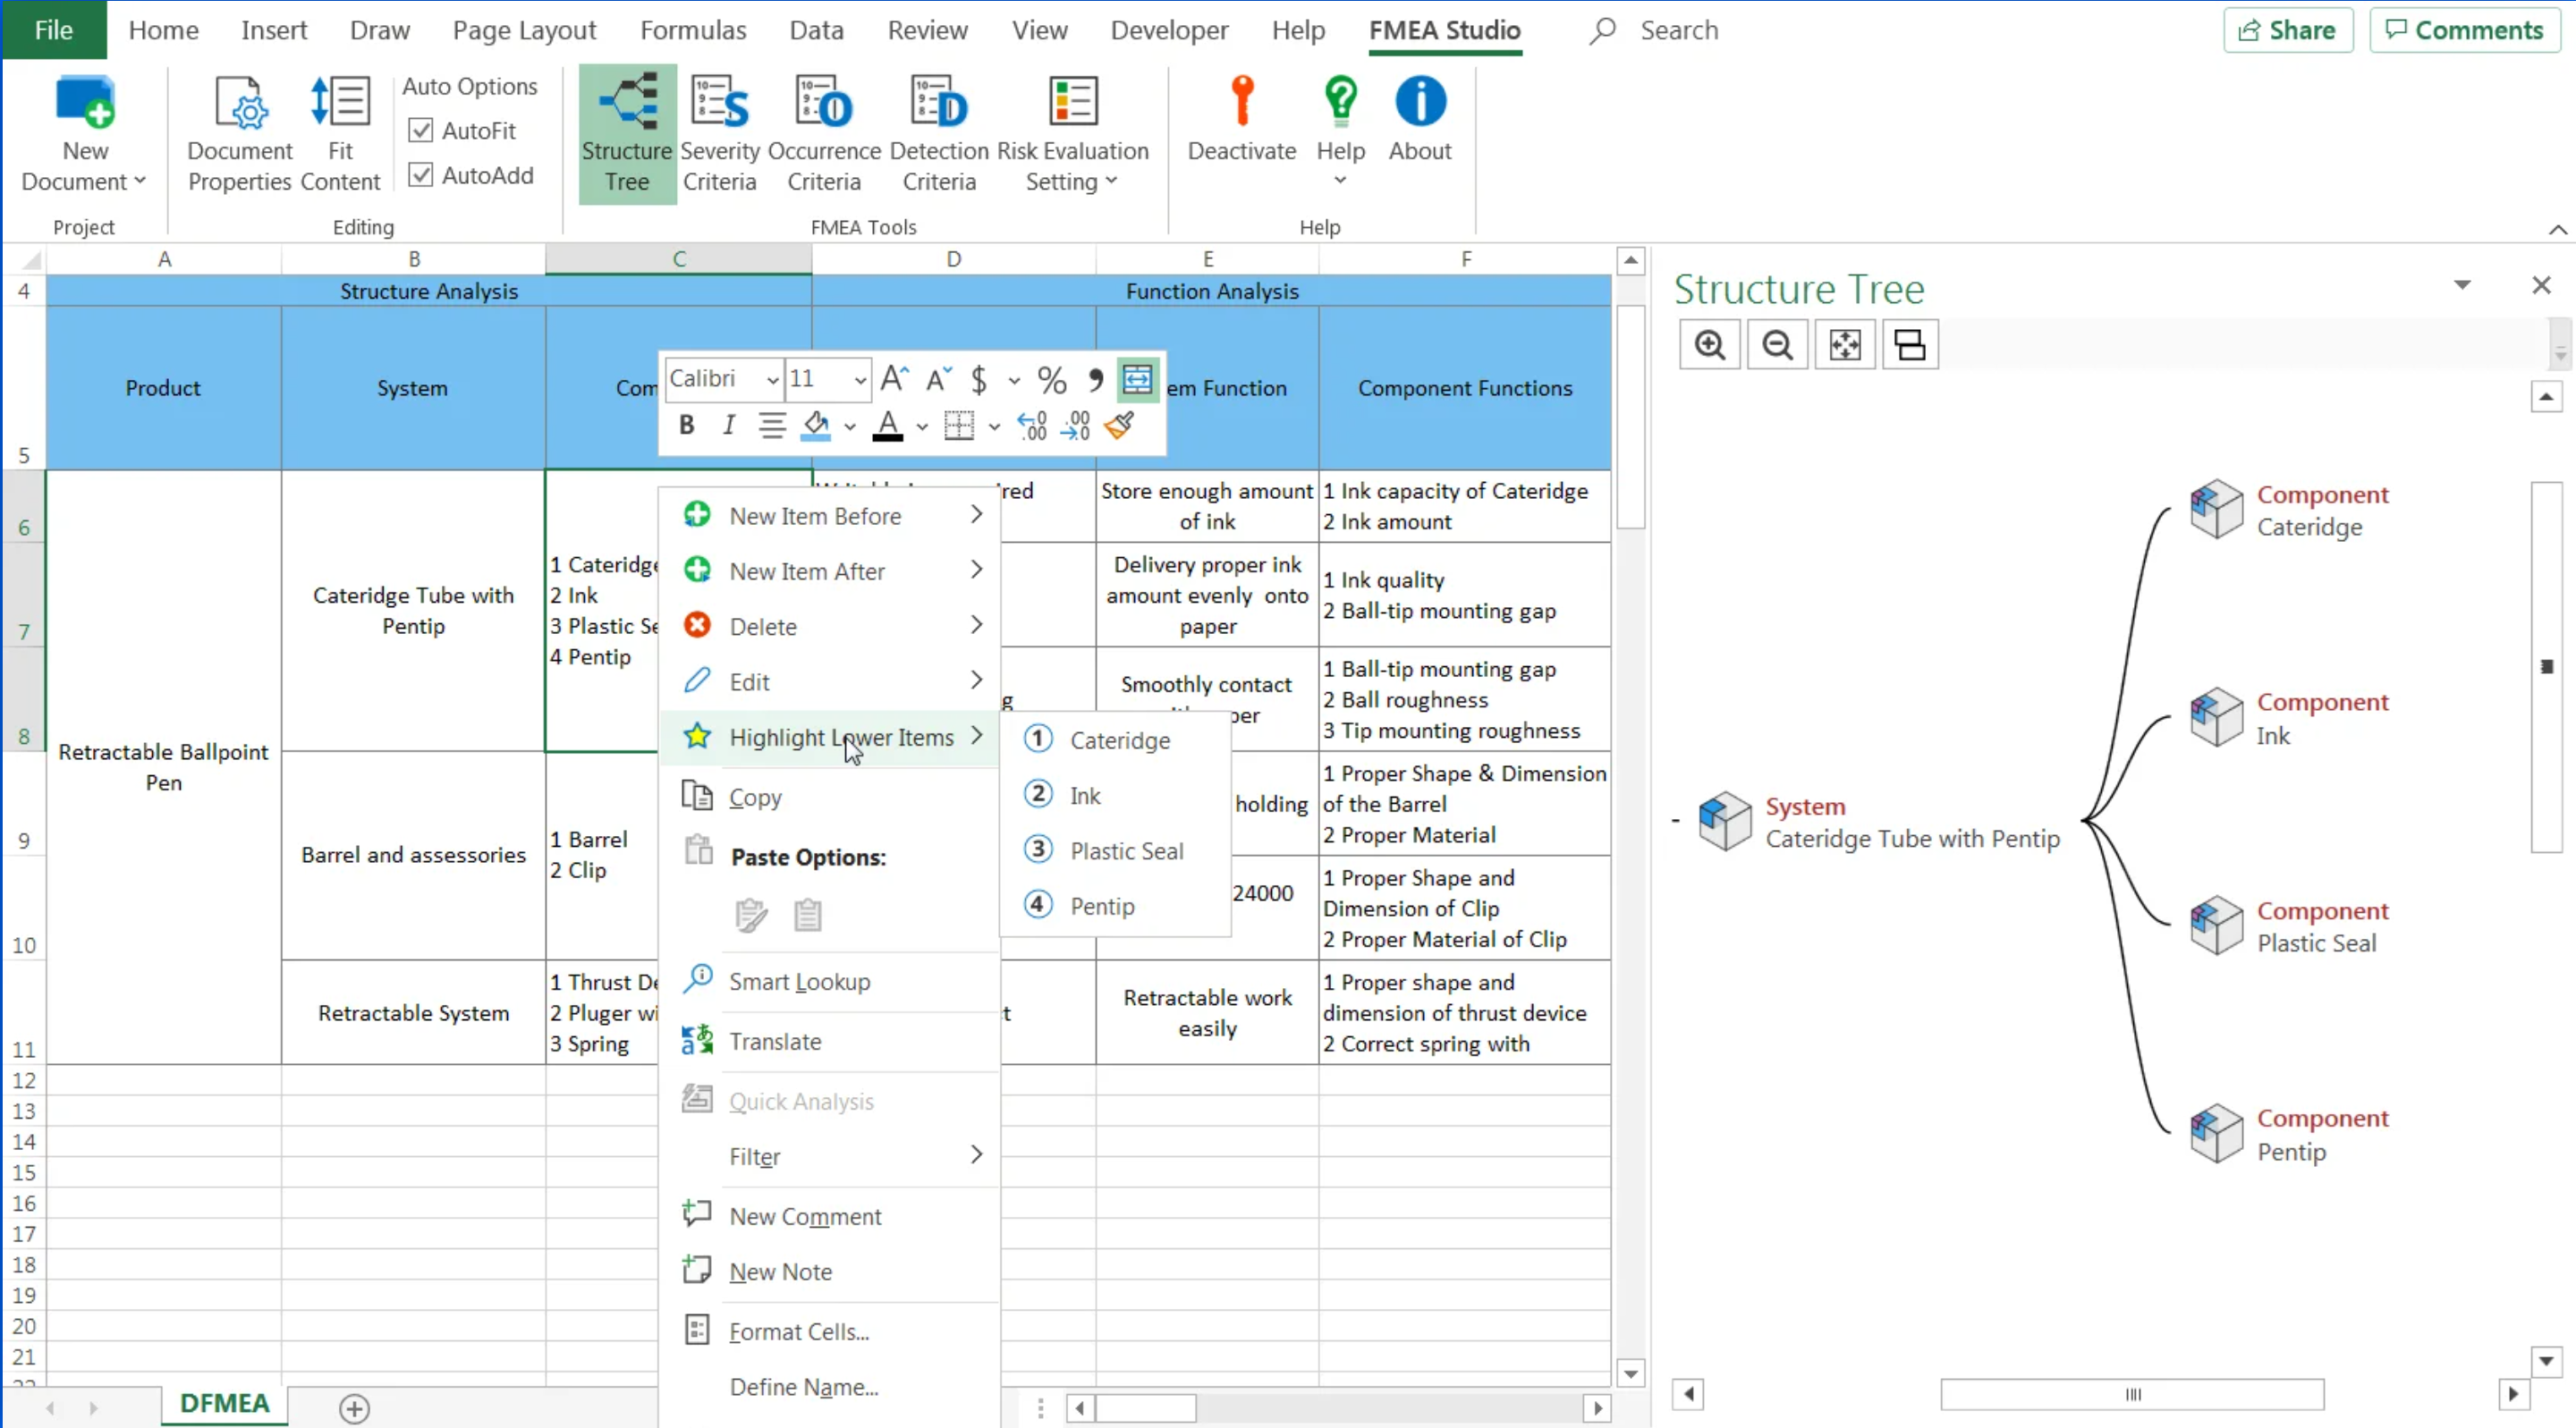
\includegraphics[width=1.0\textwidth]{Figures/iqa.PNG}
	\caption{Nástroj FMEA Sudio }
	\label{fig:iqa}
\end{figure}

FMEA Studio slouží jako nadstavba výše zmíněného způsobu tvorby analýzy pomocí tabulkového editoru. Tento nástroj slouží jako rozšíření například do programu Microsfot Excel, kde pak nabízí například několik různých šablon zaměřených zejména na Návrh a Proces. Samozřejmostí je také automatický výpočet RPN a určení AP. Uživatel má také možnost nastavení vlastních měřítek pro hodnocení atributů Význam, Výskyt a Detekce. Dokonce je možné zobrazit relace mezi daty i pomocí stromové struktury. Další užitečnou funkcí je možnost nastavení priority jednotlivých hodnotících atributů pro jednodušší určení do jakého stavu identifikováné riziko přejde. Nástroj také nabízí základní zobrazení výstupu analýzy pomocí matice rizik a grafů. Formatování je umožněno zejména pomocí hostitelského programu. Ukázku tohoto rozšíření je možné vidět na obrázku \ref{fig:iqa}
\break
\break


\subsubsection{PQ-FMEA}
PQ-FMEA je čistě desktopová aplikace pro tvorbu FMEA. Tato aplikace umožňuje tvorbu dvou základních typů(DFEMA, PFMEA) a podporuje práci s typy RPFMEA, LFMEA, MFFMEA, SwFMEA, UFMEA. Aplikace nabízí docela široké možnosti, co se týká zobrazení dat. Tabulku lze zobrazit dle standardu AIAG nebo VDA nebo jejich společné variantě. Dále lze také zobrazit kontrolní plán, což je dokument, který se z pravidla vypracovává po ukončení práce na analýze zaměřené na proces. Tento nástroj také disponuje zajímavou možností tvorby analýzy v grafickém režimu. V prvé řadě lze přepínat mezi třemi módy, které určují krok analýzy. Po výběru módu lze tvořit relace mezi prvky stylem drag\&drop. U prvního módu reprezentující strukturální analýzu je tento způsob velice účinný. Nicméně u dalších dvou módu reprezentující funkční analýzu a analýzy selhání se zobrazují v rámci sloupců kombinace atributů z předchozích kroků a celý proces je tak velice nepřehledný. Také zobrazení pomocí tabulky není úplně nejpřívětivější. V rámci kroků analýzy nejsou nijak barevně rozlišeny prvky, které spolu souvisí a pro zobrazení relací chybí slučovaní buněk tabulky. Na druhou stranu tato aplikace nabízí velikou škálu vstupních a výstupních funkcí jako je:
\begin{itemize}
    \item Nastavení vlastních měřítek pro určení hodnotících atributů spolu s možností jejich importu a exportu
    \item Tvorba logů ze setkání a přidělování úkolu jednotlivým uživatelům
    \item Zobrazení výstupních grafů analýzy, matice rizik, rozložení rizik podle AP 
    \item Tisk jednotlivých částí analýzy
    \item Možnost vyhledávání v tabulce podle klíčového slova
    \item Podporu několika světových jazyků
\end{itemize}

Jedná se tak o docela robustní nástroj s širokou škálou funkcí nicméně podle názoru autora této práce s několika základními nedostaky. Ukázku této aplikace je možné vidět na obrázku \ref{fig:pq}

\begin{figure}[h]
\centering
	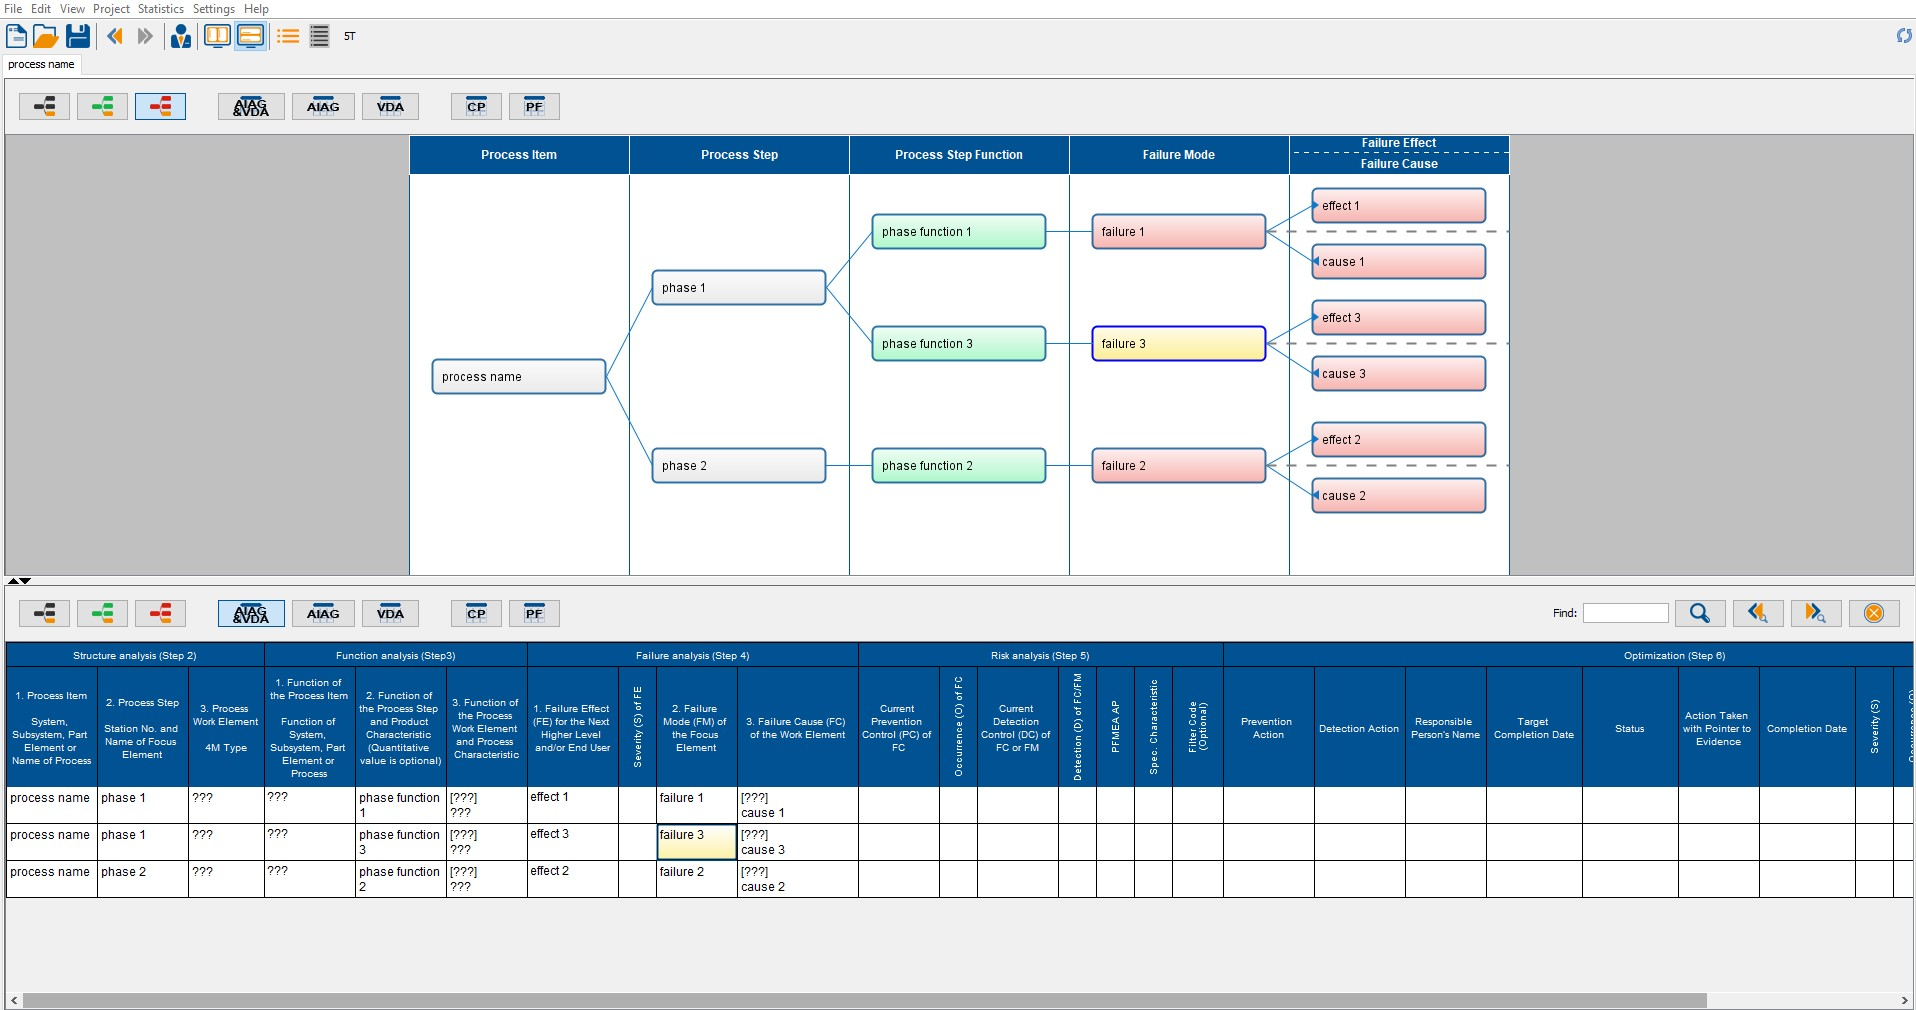
\includegraphics[width=1.0\textwidth]{Figures/pq.jpg}
	\caption{Nástroj PQ-FMEA }
	\label{fig:pq}
\end{figure}

\subsubsection{Relyence FMEA}
U předchozích dvou nástrojů se jednalo o desktopová řešení, kterým chyběla přímá podpora pro možnost sdílené práce na analýze více uživatelů. Tento problém by šel případně vyřešit za pomocí externích programů pro sdílení plochy jednoho z uživatelů a také samostatného sdílení souborů analýzy. Správným směrem se vydala společnost Relyence, která vytvořila aplikaci webovou. Tato apliakce nabízí kromě tvorby FMEA analýzy také několik dalších method z oblasti Risk Managementu jako je například Fault Tree, Reliabity Prediction apod. V rámci FMEA aplikace podporuje typy DFMEA, PFMEA, FMEA-MSR, FMECA. Tyto typy ovšem neodpovídají standardu AIAG/VGA pro automobilový průmysl. Aplikace sice nedisponuje grafickým zobrazením dat analýzy, ale nabízí opravdu komplexní možnosti práce s tabulkou. Také je možné grafické zobrazení a tvorba podpůrných souvisejích artefaktů jako je Boundary diagram nebo P-diagram. Samozřejmostí je také import a export dat analýzy do několika podporovaných formátů. Tento nástroj, narozdíl od dvou předchozích, určitým způsobem řeší správu uživatelů. Je zde možné si vytvořit uživatelský účet a ukládat si data analýzy. Zajímavostí je, že webová aplikace by měla být podle všeho také podporovat zobrazení na zařízení jako je tablet nebo dokonce mobilní zařízení. Ani u této apliakce ovšem nevypadá, že by existovali nějaké sofistikovanější možnosti společné práce na analýze. Ukázku této aplikace možné vidět na obrázku  \ref{fig:relyence}

\begin{figure}[h]
\centering
	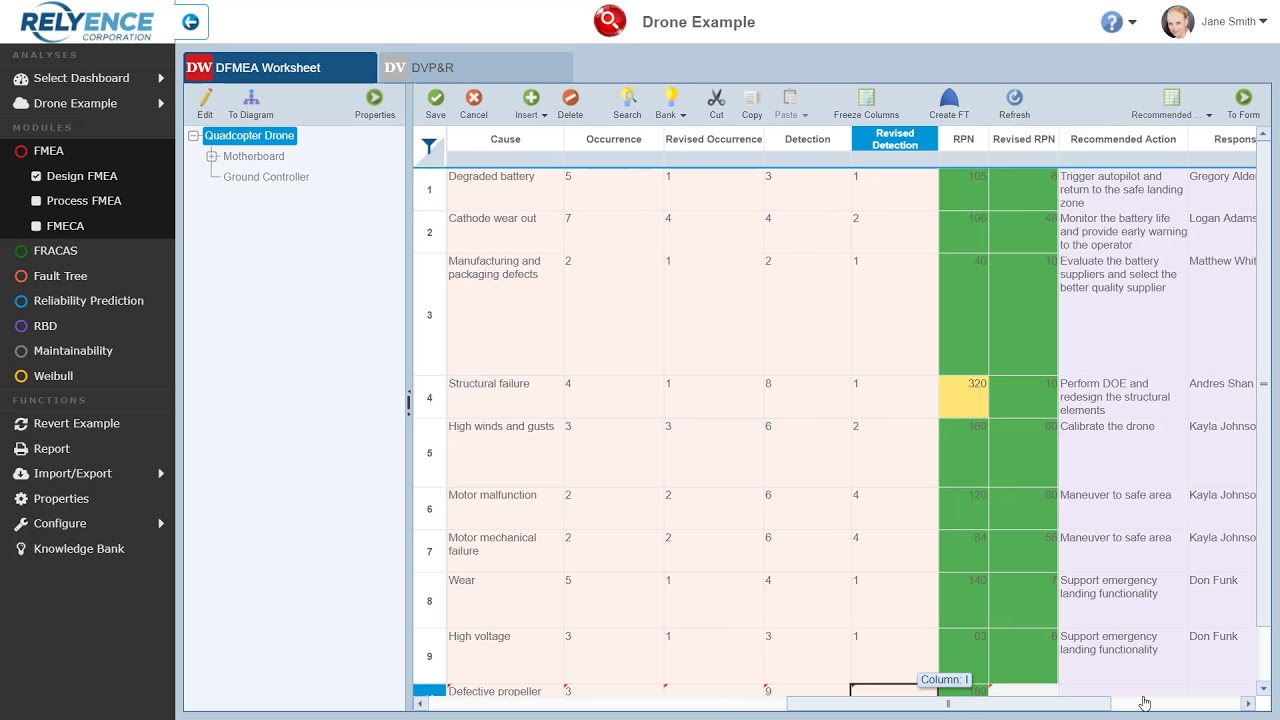
\includegraphics[width=1.0\textwidth]{Figures/relyence.jpg}
	\caption{Nástroj Relyence FMEA }
	\label{fig:relyence}
\end{figure}

\subsection{Srovnání dostupných řešení}
V této části kapitoly budou srovnány výše uvedené nástroje pro tvorbu FMEA, které jsou dostupné na trhu. Součástí tohoto srovnání bude i nástroj, který byl vytvořen v rámci této diplomové práce. Důvodem je ukazát, jak byly jednotlivé požadavky na nástroj realizovány v porovnání s ostatními komerčními produkty. Dále následuje tabulka \ref{tab:compare}, kde lze vidět na základě jakých požadavků byly nástroje posouzeny a jak je jednotlivé řešení naplňují.
\break
\break
\break
\break
\break
\break

\begin{longtable}{|p{4cm} | p{12cm} |} 
        \caption{Srovnání dostupných řešení}
\label{tab:compare}
         \hline
& \textbf{1. Tvorba analýzy podporující typy DFMEA, PFMEA,...} \\ \hline
 FMEA Studio &	DFMEA,PFMEA, Software FMEA  \\ 
 PQ-FMEA &	 DFMEA,PFMEA  \\ 
 Relyence FMEA &	 DFMEA,PFMEA, FMECA, FMEA-MSR  \\ 
Vlastní řešení &	 DFMEA,PFMEA \\ \hline

& \textbf{2. Zobrazení dat analýzy pomocí textové tabulky.}  \\ \hline
 FMEA Studio &	Rozšíření tabulkového editoru + přidané některé vlastní funkce, správné slučování buněk, nedostatečné barevné rozlišení souvisejících atributů.  \\ 
 PQ-FMEA &	 Různé možností zobrazení, špatné slučování buněk, nedostatečné barevné rozlišení souvisejích atributů.  \\ 
 Relyence FMEA &	 Pokročilé funkce práce s tabulkou, správné slučování buněk na základně relací mezi atributy.  \\ 
Vlastní řešení &	 Zobrazení a následně i editace dat tabulky, zobrazení relací slučováním buněk, rozšířené barevné rozlišení souvosejích atributů s možností označení jednotlivých prvků ze strukturální analýzy. \\ \hline

& \textbf{3. Zobrazení dat analýzy v grafickém režimu.} \\ \hline
 FMEA Studio &	 Možnost zobrazit strukturu dat v jednotlivých krocích na samostatném panelu, přidávání i editace prvků.\\ 
 PQ-FMEA & Náhled i tvorba pomocí tří módu zobrazení stromovou strukturou, lehce nepřehledné v rámci některých módů, tvorba stylem drag\&drop a úpravá prvků.  \\ 
 Relyence FMEA &	 NE  \\ 
Vlastní řešení &	 Možnost tvorby stromové struktury, následně přidávání funkcí a selhání jednotlivým prvků ze struktury pomocí modálních oken, zoom, skrytí/zobrazení potomků. \\ \hline

& \textbf{4. Soubežná práce více uživatelů.} \\ \hline
 FMEA Studio &	Za pomocí externího software + sdílení souboru analýzy.  \\ 
 PQ-FMEA &	 Za pomocí externího software + sdílení souboru analýzy. \\ 
 Relyence FMEA &	  Základní práce s uživatelskými účty, jinak pomocí externího SW + sdílení souborů.  \\ 
Vlastní řešení &	 Možnost připojení několika uživatelů do skupin na základě stejného odkazu a sdílení prováděných změn v reálném čase. Registrace a přihlašování uživatelů. \\ \hline

& \textbf{5. Možnost export a importu dat analýzy. } \\ \hline
 FMEA Studio &	Pouze ukládání a načítaní souboru tabulkového editoru.  \\ 
 PQ-FMEA &	  Ukládání a načítání dat analýzy do vlastního formátu, import a export nastavení vlastních měřítek pro hodnocení.   \\ 
 Relyence FMEA &	 Ukládání a načítání dat analýzy do vlastního formátu.  \\ 
Vlastní řešení &	 Ukládání a načítaní dat analýzy do JSON formátu, export do formátu .xls, .png.\\ \hline

& \textbf{6. Další podpůrné funkce(nastavení vlastních měřítek hodnocení, grafy na výstupu)} \\ \hline
 FMEA Studio &	Nastavení vlastních měřítek pro hodcnocení, hranic pro hodnocení rizik, výstupní grafy a matice rizik, flow diagram,...  \\ 
 PQ-FMEA &	 Nastavení vlastních měřítek pro hodcnocení, výstupní grafy a matice rizik, tisk formulářů, logování a přidělování úkolů uživatelům.  \\ 
 Relyence FMEA &	  Možnost importu a tvorby několika souvisejících diagramů. \\ 
Vlastní řešení &	  Nastavení vlastních měřítek pro hodnocení, tvorba logů ze setkání, kontrola dokončení všech nalezených rizik. \\ \hline
\end{longtable}

Závěrem tohoto popisu lze říci, že ač nalezené nástroje obsahují několik dostupných typů FMEA, různých možností nastavení projektů, výstupních grafů a matic, tak postrádají jednu ze základních funkcí a to umožnit týmu provádějící analýzu souběžnou a efektivní práci na analýze přímo skrze používáný nástroj. To je nesporná výhoda nástroje, který byl vytvořen v rámci této práce. Další výhodou je, že vytvořený nástroj celkem jasně sdružuje atributy, které spolu souvisí, kdy u jiných nástrojů nejsou jednotlivé souvislosti hned na první pohled jasné. Následuje kapitola \ref{sec:navrh}, která již bude zaměřena vyvýjený nástroj, nejdříve jeho návrh a architekturu. 
 
\chapter{Architektura a návrh aplikace}
\label{sec:navrh}
Tato kapitola bude zaměřena na popis architektury a zvolených technologií, způsobu uložení dat a návrhu uživatelského rohraní. U jednotlivých popisů bude uvedeno z jakých důvodu byly jednotlivé návrhové rozhodnutí učiněny. 

\section{Architektura systému}
Vzhledem k tomu, že byl jeden z hlavních požadavků na vyvýjený nástroj, umožnit přístup k aplikaci jedním či více uživateli zároveň, jevila se jako nejlepší možnost vytvořit webovou aplikaci dostupnou na zařízeních disponující webovým prohlížečem a připojením k internetu. Webové aplikace fungují na známé a rozšířené architektuře klient-server. Tato architektura dělí systém na klienta(uživatele) a server, kteří spolu komunikují, v případě webových aplikací, skrze internetový protokol HTTP. Zjednodušeně by se tato komunikace dala popsat jako série požadavků klienta a odpovědí ze strany serveru. 

Ještě před několika lety tento způsob tvořil základ webových stránek a aplikací. Tato komunikace sebou bohužel přínáší i jisté nevýhody v podobě delší odezvy webových aplikací, nutnosti obnovení zobrazené stránky apod. Jednotlivé události vyvolané uživatelem se musí řešit na straně serveru, ten vygeneruje odpověď ve formě html souboru, který si uživatel následně zobrazí v prohlížeči. Moderní způsob tvorby webových aplikací je minimalizace této komunikace a přenechání zpracování požadavků na straně zařízení klienta. To je z pravidla umožněno díky Javascriptu, což je skriptovací jazyk, jehož běhovým prostředím je právě webový prohlížeč. Javascript jako takový je jazyk, ve kterém se relativně dobře a rychle tvoří jednoduché skripty, nicméně pro větší a komplexnější projekty byly vytvořeny jeho nadstavby a rozšíření, které zjednodušují vývoj, efektivitu a správu aplikací. 

Jak je vidět na obrázku \ref{fig:architecture}, který znázorňuje diagram nasazení, tak bylo použito hned několik těchto rozšíření. Na tomto obrázku je kromě klienta a webového serveru ještě znázorněn server sloužící pro persistentní uložení dat(databáze). Zde je komunikace rodělena přímo na požadavky typu CRUD neboli všchny operace, které se provádějí se záznamy databáze a odpovědi ve specifickém formátu pro danou technologii. Nicméně se jedná stále o komunikaci pomocí protokolu HTTP stejně jako v případě klienta a webového serveru. Dále je zde také nastíněno rozdělení dnešních webových aplikací a to na front-end a back-end. Rovnou by bylo dobré říci, že i když je zde webový server a back-end znázorněn opticky větší, tak se podstatná část úloh zpracovává na straně klienta. 

\begin{figure}[h]
\centering
	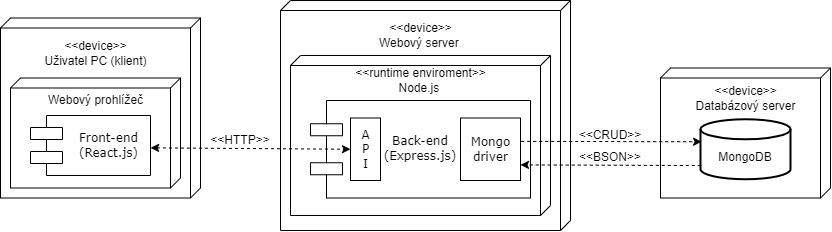
\includegraphics[width=1.0\textwidth]{Figures/deploymentDiagram.png}
	\caption{Diagram nasazení}
	\label{fig:architecture}
\end{figure}

\section{Použité technologie}
V této sekci boudou popsány technologie, které byly použit pro vývoj nástroje pro tvorbu FMEA. Jak bylo nastíněno v předchozí kapitole, tak byl zvolen přístup pro aplikaci, která zpracovává uživatelské požadavky převážně na straně klienta. Tyto aplikace se také nazývají SPA(Single Page Application). V praxi se pro tento typ vývoje používají především rozšíření založené na Javascriptu. I z toho důvodu byl zvolen pro vývoj tzv. MERN stack, tedy použití technologií: MongoDB, Express, React, Node. 
\subsection{React}
\label{subsection:react}
\cite{react}Prvním rozšířením nebo též frameworkem je React, kterým je jedním z nejpoužívanějších frameworků pro vývoj webových aplikací na straně klienta. Stejně jako ostatní populární javascriptové frameworky, jako například Angular nebo Vue, tak se aplikace dělí na jednotlivé bloky, které se nazývají komponenty. Komponenty spolu přinášejí obdobné výhody jako když hovoříme o třídách a objektech v objektově orientovaném programování. Zápisů komponent je více, ale obecně obsahují stav, vlastní programovou logiku v podobě metod a návratovou funkci ve formě html elementu.  

S tím také souvisí přístup, který se používá v Reactu a to je virtuální DOM. DOM je vlastně objektová reprezetace stromové struktury elementů, kterou obsahuje každý HTML soubor. Tento strom se běžně používá pro manipulaci s elementy pomocí Javascriptu. React přišel s nápadem, kdy interně pracuje s vlastní verzí této struktury a při změnách na základě události na stránce provádí aktualizace pouze ovlivněných komponent danou změnou. Určení se provádí na základě porovnání původních a aktualizovaných DOM struktur. Také závisí i na tom, jak programátor danou aplikaci dekomponuje. 

Dalším vlastností Reactu je možnost komibinace html kódu a programové logiky. To je skutečnost, která je řešena i v jiných frameworcích pro web. V Reactu se jedná o vlastní formát souboru s příponou JSX, která umožňuje uvnitř HTML kódu komponent psát Javascript pomocí kombinace symbolu '\$' a složených závorek. Nejčastěji se toto využívá při vložení hodnoty proměnných nebo například při použití cyklu, který v každé iteraci vytváří nějakou sadu html elementů. 

\subsection{Node}
\cite{node}Node je běhovým prostředím pro Javascript na straně serveru postavený na Chrome V8 Javascript enginu. Javascript je navržen pro běh v prohlížeči a proto byl vytvořen Node, který umožňuje vytvářet aplikace na straně serveru v tomto jazyku. Architektura Nodu je založena na tzv. smyčce událostí, kdy jsou postupně zachytávány uživatelské požadavky v rámci jednoho vlákna a dále přiděleny jednotlivým asynchroním vláknům. 

Další velice důležitou součástí Nodu je NPM(Node Package Manager), což je balíčkovací ekosystém, který umožňuje vývojáři přidávat balíčky(knihovny) do svého projektu pomocí konzole. Jedná se o jednu z největších databází knihoven na světě. V době psaní tohoto textu se počet odahaduje na více než 2.1 milionů balíčků. Díky tomuto faktu je vývoj webových stránek opravdu zjednodušen. V praxi se dá postupovat tak, že si vývojář navrhne strukturu své aplikace a pak prakticky pro jakoukoli funkcionalitu chce, si může vybrat z nabídky několika balíčků, které jsou k dispozici. Vybraný balíček si pak jednoduše nainstaluje pomocí příkazu v konzoli a pomocí dostupné dokumentaci pouze přidá požadavanou komponentu, metodu atd. Seznam všech balíčku obsahuje soubor s názvem "package.json", který také vyjadřuje seznam závislostí.  

\subsection{Express}
\cite{express}Express je rychlý, nezávislý framework pro Node zjednodušující vývoj aplikací na straně serveru. Ikdyž jsou snahy o to přesunout většinu zpracování na klienta, tak je stále potřeba komunikace se serverem například v případě prací se záznamy v databázi. Tato komunikace probíhá na základě HTTP protokolu a také pomocí základních metod, které se používají při tvorbě tzv. API, které slouží jako komunikační bod pro klienta. Nejčastěji používáné metody jsou GET, POST, PUT, DELETE. Express umožňuje psaní metod pro zpracování těchto požadavků. Metody obsahují v parametrech vždy atribut pro definici požadavku a odpověď, která slouží jako navratová hodnota.   

\subsection{MongoDB}
\cite{mongo}Pro persistentní uložení dat byla nakonec vybrána No-SQL databáze MongoDB spolu s Mongoose ODM. Důvod výběru Mongo databáze i krátký popis již byl zmíněn v kapitole \ref{sec:pozadavekMongo}, kde byl vysvětlen důvod zamítnutí systémového požadavku na tvorbu relační databáze. 

Mongoose je javascriptová knihovna, která vytváří propojení mezi MongoDB a běhovým prostředí Node. Označení ODM se používá pro databáze založené na ukládání dokumentů oproti klasickému ORM používaném v relačních databázích. Výhoda Mongoose je, že nabízí několik základních metod pro připojení k databázovému serveru, vytvoření schémat pro ukládání dokumentů a metod pro jejich manipulaci. 

\section{Návrh datové vrstvy}
Tato sekce se bude zabývat popisem a ukázkou toho, jak se v aplikaci pracuje s daty. Jak je možné vidět na obrázku \ref{fig:db} znázorňující relační vztahy čistě v rámci atributů analýzy, tak se jedná o relativně dosti provázanou strukturu. Zjednodušeně diagram obsahuje tabulku pro hlavičku analýzy, dále se následující tři kroky analýzy skládájí vždy ze tří úrovní, kdy spolu jednotlivé úrovně mezi sebou navzájem souvisí. Pátý a šestý krok analýzy je součástí třetí úrovně analýzy selhání, která je s ní pevně spjata. V návrhu je vidět, že mezi atributy převládají vazby 1-N a byly detailněji popsány již v teoretické části práce. Co se týká atributů objektů, tak prakticky každý objekt obsahuje atribut ID pro identifikaci a Name, který odpovídá hodnotě vyplněného pole hodnotícím týmem. Pro zajímvaost ještě možná dobré zmínit atribut Initial Severity(Vážnost), který se vyskytuje u selhání druhé úrovně narozdíl od ostatních hodnotících atributů. Je to z toho důvodu, že jedna hodnota tohoto atributu narozdíl od ostatních může odpovídat více objektům třetí úrovně. Nakonec se tento atribut vyskytuje i v rámci formuláře analýzy v odišném kroku analýzy narozdíl od atributů Výskyt a Detekce. Na závěr tohoto popisu je potřeba se krátce zmínit k dvěma typům analýzy: DFMEA a PFMEA. Oba dva tyto typy mají totožnou strukturu, co se týká počtu atributů, ale rozdílné názvy atributů hlavně v rámci analýzy struktury a funkcí a proto jsou v diagramu uvedeny obecně názvy objektů spolu s číslem označujícím úroveň. 

Návrh toho, jak ukládat data se ze začátku zdál docela jako komplikovanější úkol. Důvodem byl výběr knihovny, která slouží pro zobrazení stromové struktury v rámci grafického zobrazení analýzy. Pro práci s touto knihovnou je potřeba data udržovat v několikanásobně zanořeném objektu (viz. \ref{src:data}, který obsahuje atribut 'children'. Problém byl, jak vytvořit výše popsané relace v této datové struktuře Nakonec se toto podařilo pomocí toho, že v rámci objektu lze jeho atributy uložit jako pole dalších objektů, tím pádem šlo vytvořit tímto způsobem požadované vazby 1-N. Jedinou nevýhodou tohoto řešení bylo to, že některé záznamy musí být redundatní a operace aktualizace a mazání byly taktéž trochu složitější. Nicméně nespornou výhodou toho, že se podařilo spravovat všechna data v rámci jednoho zanořeného objektu bylo to, že se dala velice efektivně využít databáze založená na ukládání dat pomocí dokumentů. Pomocí tohoto způsobu uložení dat, lze rovnou uložit celý objekt bez jakékoli nutnosti transformace dat např. pomocí návrhového vzoru DTO, který slouží právě pro podobné situace. 

\begin{figure}[H]
\centering
	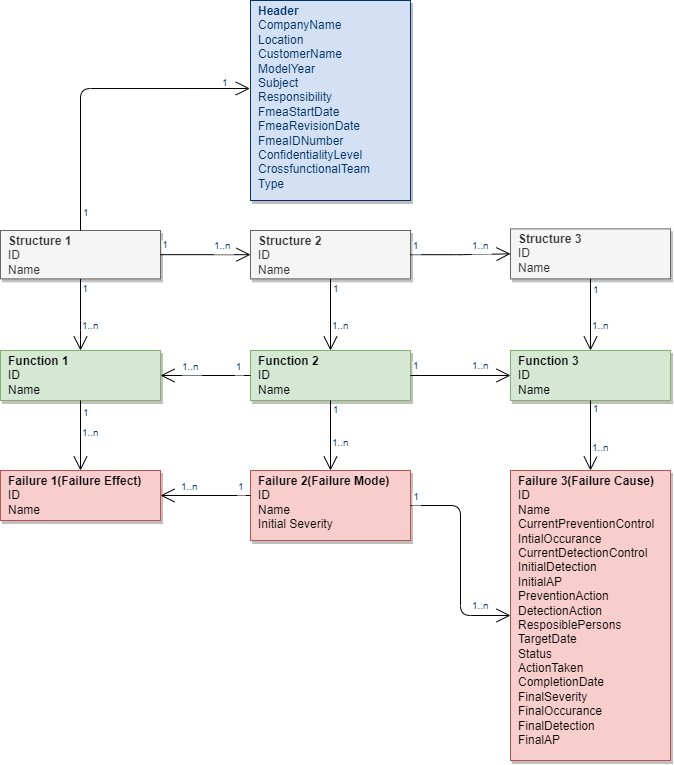
\includegraphics[width=1.0\textwidth]{Figures/db_model.png}
	\caption{Konceptuální diagram }
	\label{fig:db}
\end{figure}

\section{Návrh uživatelského rozhraní}
Poslední část této kapitoly bude zaměřena na Návrh uživatelského rozhraní. Jak bylo řečeno v úvodu kapitoly, tak bude snaha vyvynout tzv. Single Page Application. A to nejen z pohledu zpracování požadavků, ale také shodou okolností z pohledu uživatelského rohraní. Vize je taková, že bude existovat jedna stránka obsahující grafický i textový pohled na analýzu. Úpravy atributů a ostatní funkce budou vyřešeny v rámci modálních oken. Uživatel tak bude mít všechny funkce na jedné stránce bez nutnosti přecházet na jiné odkazy v rámci webu. 

Důležitým rozhodnutím při návrhu uživatelského rozhraní bylo jaký zvolit formát tabulky. Možností existuje více, ale v základu se běžně používá řešení, kdy jsou všechny kroky tabulky za sebou v řádku. Problém v tomto zobrazení je ten, že se velice obtížně zobrazují všechny relace v jednom řádku při současném slučování buněk. Zároveň jednotlivé atributy mezi sebou v rámci kroků analýzy souvisí, což v nemusí být v řádku bez barevného označení také hned zřejmé. Proto bylo nakonec zvoleno jedno z novějších zobrazení, které je uvedeno například v posledním vydání přiručky FMEA pro automobilový průmysl.\cite{handbookExample} V rámci tohoto zobrazení jsou první tři kroky analýzy nad sebou, což výrazně zvyšuje čitelnost souvisejích prvků. Zbytek kroků vycházející z odhalených přičin selhání je již pak bez problému zobrazen v řádku. Náhled tohoto formátu zobrazení lze vidět na obrázku \ref{fig:ui}.

\begin{figure}[h]
\centering
	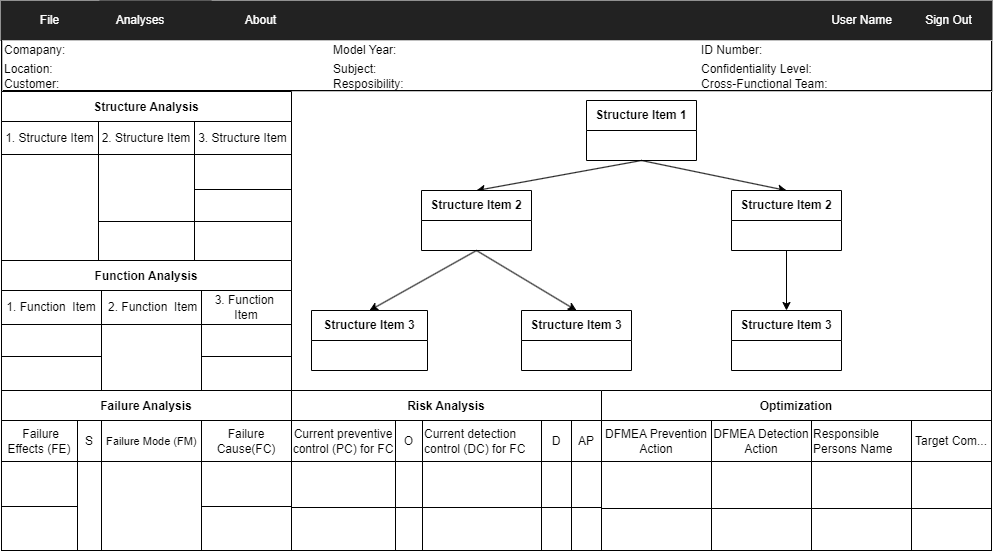
\includegraphics[width=1.0\textwidth]{Figures/mockup3.png}
	\caption{Návrh uživatelského rozhraní }
	\label{fig:ui}
\end{figure}
\chapter{Implemetace a testování}
\label{sec:implementace}
Tato kapitola se bude zabývat popisem implementace nástroje pro tvorbu FMEA. Na základě daných skutečností popsaných v předchozí kapitole byla vytvořena webová aplikace. Základní rozdělení této aplikace je na front-end(klientská část) a back-end(serverová část) . Ač je tato aplikace postavena převážně na straně klienta, tak bude následující popis obsahovat i kapitolu pro popis serverové části.

\section{Backend}
Požadavků, které se v této aplikaci zpracovávají na straně serveru není mnoho. Nicméně to k k čemu se serverová část využívá by se dalo zúžit na dvě oblasti: 
\begin{itemize}
    \item Ukládání a načítání analýzy
    \item Sdílení dat mezi uživateli
\end{itemize}

\subsection{Ukládání a načítání analýzy}
Pro persistentní uložení dat analýzy se používá MongoDB, kde je objekt analýzy uložen v nezměněném stavu jako součást uloženého dokumentu. Struktura objektu obsahující data nalýzy je součástí přílohy(\ref{src:data}) této diplomové práce. Struktura obsahuje zejména základní atributy pro ukázku zanořenosti objektu, některé méně důležité atributy jsou zjednodušeny nebo vynechány. Toto ukládání je provedeno pouze na základě vyvolané události od uživatele. Zároveň platí, že pro persistentní ukládání dat analýzy musí být uživatel přihlášen. V opačném případě mu nejsou tyto možnosti zobrazeny v rámci menu. Toto platí i z toho důvodu, že každý záznam databáze je přiřazen určitému uživateli. Přihlášený uživatel si poté může načítat své uložené analýzy. Pro manipulaci s databází je použit ODM framework Mongoose, v rámci kterého je potřeba definovat model ukládaných dokumentů. Tento model obsahuje tyto parametry: 
\begin{itemize}
    \item \textbf{ID} - Unikátní identifikační číslo dokumentu. Pro vytvoření tohoto čísla se používá knihovna uuidv4 \cite{uuid}, která generuje náhodný 36-místný unikátní řetězec znáků složených z písmen a-z a číslic 0-9.  
    \item \textbf{data} - Objekt, který obsahuje všechna potřebná data analýzy v původním formátu.
    \item \textbf{ownerID} - Identifikační číslo přihlášeného uživatele. Toto číslo má každý registrovaný uživatel v rámci platformy Firebase, která se používá pro práci s uživatelskými účty a bude popsána později. 
\end{itemize}

Pro připojení k databázi se používá metoda \textit{mongoose.connect(connectionString)}, jejímž parametrem je řetězec obsahující odkaz na databázový server a případně údaje k uživatelskému účtu v rámci MongoDB. Tyto údaje nejsou součástí zdrojového kódu, ale jsou získány na základě tzv. proměnných prostředí. Pro manipulaci dokumentů se pak používají asynchroní metody, které lze zavolat na objekt vytvořený v rámci modelu. Tyto metody jsou: 
    
\begin{itemize}
    \item \textit{create(object)} - Tato metoda se používá pro vytvoření dokumentu v rámci modelu pro analýzu. Tato metoda přijímá jako parametr objekt, jehož atributy, byly definovány v předchozím výčtu. 
    \item \textit{findOne(object)} - Metoda pro nalezení jednoho dokumentu v kolekci dokumentů. Metoda přijímá objekt, jehož atributem je nejčastěji pouze id hledaného dokumentu. 
    \item \textit{find(object)} - Pomocí této metody lze nalézt v kolekci dokumentu jeden a více dokumentů. Parametrem je objekt obsahující, v tomto případě, identifikační číslo uživatele.   
    \item \textit{deleteOne(object)} - Tato metoda slouží pro smazání jednoho dokumentu v kolekci na základě poskytnutého id, které je atributem objektu v parametru metody. 
    \item Zvláštností ze strany použitého ODM je, že neposkytuje uspokojivé řešení pro aktualizaci dokumentu. Jediná možnost, která funguje pro aktualizaci je použití metod, které dokážou například přidat jeden atribut k dokumentu. Bohužel nebyl nalezen jednoduchý způsob nebo metoda, jak aktualizovat celý dokument jako takový. Což je vlastnost, která je v rámci vyvůjeného nástroje žádoucí. Změny totiž postihují často několik atributů objektu analýzy. Řešení bylo nakonec použití kombinace metody pro smazání a vytvoření nového aktualizovaného záznamu, což je způsob účinný, ale ne zrovna efektivní.  
\end{itemize}

\subsection{Sdílení dat mezi uživateli}
Další zajímavější oblastí, která je řešena na straně serveru je sdílení dat mezi uživateli v reálném čase. Je to jedna z hlavních funkcí, na které je aplikace postavena umožňující efektivní práci týmu provádějící analýzu. Tuto funkcionalitu zajišťuje knihovna Socket.IO. 

Socket.IO je knihovna, která umoňuje rychlou, obousměrnou komunikaci mezi klientem a serverm založenou na eventech. \cite{socketIO} Tato knihovna je postavena na komunikačním protokolu WebSocket, což je protokol umoňující navázání a udržení komunikace mezi klientem a serverem. Socket.IO také využívá pro realizaci metod GET(získání dat ze serveru) a POST(odeslání dat na server) tzv. HTTP long-polling. Jedná se o alternativní metodu, která byla využívána v dobách, kdy prohlížeče komunikaci přes protokol WebSocket nepodporovali. Velikou výhodou obou těchto metod je, že nabízí alternativu oproti standardní komunikaci mezi klientem a serverem, kdy je navázáno spojení, vytvořen požadavek, odeslání odpovědi a ukončení spojení. V tomto případě lze po navázání spojení vytvářet několik požadavků bez ztráty spojení.

Další výhodou oproti samotnému použití řešení používající pouze protkol WebSocker je, že Socket.IO nabízí řešení pro některé základní problémy, které se řeší při sdílení dat mezi uživateli. Příkladem je rozdělení uživatelů do skupin na základě ID a broadcast prováděných změn mezi ostatní účastníky skupiny. Příklad takovéhoto rozdělení je vidět na obrázku \ref{fig:rooms}. 

\begin{figure}[h]
\centering
	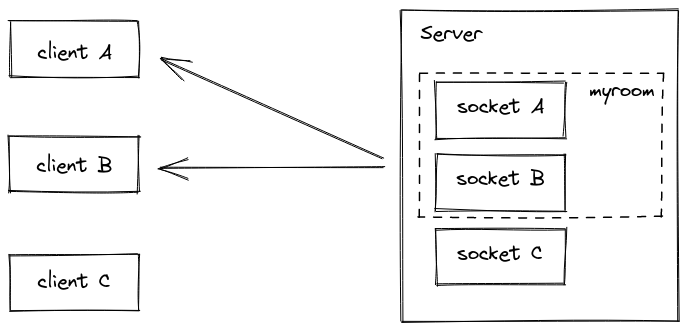
\includegraphics[width=1.0\textwidth]{Figures/rooms.png}
	\caption{Skupiny v rámci Socket.IO}
	\label{fig:rooms}
\end{figure}

Co se týká implementace této komunikace na straně serveru, tak se úvodem inicializuje server použitím metody z knihovny \uv{socket-io} \  s parametry číslo portu a volitelným objektem, který se používá pro zamezení chyby CORS, která nastává v případě přístupu k adrese z jiné domény. Dále se pracuje s událostmi a to tím způsobem, že klient vytváří různé typy událostí a server naopak čeká na několik typů těchto události a patřičně na ně reaguje. Zde je seznam událostí, se kterými se pracuje v rámci komunikace mezi klientem a serverem: 

\begin{itemize}
    \item \textbf{connection} - Inicializační událost, která informuje server o připojení nového uživatele.
    \item \textbf{get-analysis} - Tato událost je vyvolána pro první načtení dat analýzy. Parametrem této metody je vygenerované nové ID, které je obsaženo v url odkazu, a které se dále použije jako ID vytvořené místnosti připojených uživatelů. Uživatel, který vyvolal událost \textbf{connection} je přidán do skupiny s tímto ID pomocí metody \textit{join} poskytované knihovnou. 
    \item \textbf{send-changes} - Další událost se pak již stará o sdílení změn provedených uživateli. Server reaguje na tuto událost rozesláním přijatých dat v rámci vyvolání vlastní události \textbf{receive-changes}, na jejíž zpracování zase čeká klient. Tato událost je zaslána všem uživatelům v rámci skupiny kromě uživatele, který vyvolal původní událost. 
    \item \textbf{save-analysis} - Další událost se již týká práce s dokumenty v databázi. První událost je reakce na žádost uživatele pro uložení nové analýzy. Data analýzy jsou parametrem události.  
    \item \textbf{update-analysis} - Další se pak stará již o aktualizaci existujícího dokumentu metodou popsanou v předchozí kapitole. Data jsou zde také součástí parametru události. 
      \item \textbf{load-analysis} - Poslední metoda slouží pro načtení všech uložených analýz uživatelem. Parametrem této události je ID uživatele. Server jako reakci na tuto událost vyvolá vlastní událost \textbf{receive-analyses} obsahující kolekci načtených dat. 
\end{itemize}

Implementace na straně klienta je taková, že se použije metoda io z knihovny \uv{socket.io-client}, která má jako parametr url adresu serveru. Metoda vrácí objekt, který se pak používá ve všech komponentách, které mění data aplikace. Pomocí tohto objektu se pak vyvolávají a zachycují výše uvedené události. 



\section{Frontend}
V této kapitole bude ukázána hlavní část aplikace a to klientská část, se kterou interaguje uživatel přístupující k webové aplikaci. Postupně budou popsány jednotlivé části aplikace jak z uživatelského tak implementačního úhlu pohledu. 

\subsection{Struktura aplikace}
Jak již bylo zmíněno v kapitole \ref{subsection:react}, tak při použití Reactu vývojář tvoří strukturu aplikace pomocí komponent. Na obráku \ref{fig:structure} je vidět hlavní stránka aplikace rozdělena do těchto komponent. Zde je výčet těchto komponent rozlišených v rámci obrázku barevnými obdelníky odpovídající barvě textu: 

\begin{itemize}
    \item \textcolor{blue}{App} - Hlavní komponenta aplikace, která obsahuje všechny ostatní viditelné komponenty. Komponenta je pouze součástí komponent, které jsou zodpovědné za směrování url odkazů a komponenta v rámci balíčku React-redux, což je knihovna, která slouží pro správu globálního stavu dat aplikace a bude popsána později.  
    \item \textcolor{green}{Navigation} - Komponenta, která vystupuje v aplikaci jako menu. Toto menu je víceúrovňové a obsahuje položky pro manipulaci s dokemntem analýzy, dále popdpůrné funkce při tvorbě analýzy a napravo sekci pro registraci a přihlášení k uživatelskému účtu. 
    \item \textcolor{red}{Header} - Tato komponenta obsahuje první krok analýzy a to hlavičku obsahující základní informace o analýze. Údaje se zadávají do textových polí, které disponují animací, která při kliknutí popisný text zobrazí na vrchní stranu elementu a umožní zadávání textových hodnot. Při zadání alespoň jedné hodnoty v rámci hlavičky zůstavají elementy ve stavu pro zadávání textu.  
    \item \textbf{TreeGraph} - Jedná se o jednu z hlavních komponent aplikace, která slouží pro grafické zobrazení náhledu analýzy. Jak je vidět, tak lze v rámci této komponenty tvořit stromovou strukturu analyzovaného produktu. Součástí komponety je i ukazatel rozsahu přiblížení nacházející se na spodní straně komponenty. Detailněji bude tato komponenta popsána v kapitole \ref{sec:grafika} zaměřené na grafický náhled aplikace. 
    \item Následují komponety sloužící jako textový náhled na analýzu. Ač se může zdát, že tabulkový náhled tvoří jeden tabulkový element, tak při tomto zobrazení to není úplně možné. Proto je tabulka rozdělena na komponety \textcolor{pink}{VerticalTable} a \textcolor{magenta}{HorizontalTable}. \textcolor{pink}{VerticalTable} obsahuje první dva kroky analýzy: strukturální a fuknční analýzu. \textcolor{magenta}{HorizontalTable} pak obsahuje analýzu selhání a rizik a optimalizační kroky. Jak je vidět tak v rámci kroků analýzy, kde se mezi atributy tvoří relace, tak jsou tyto vztahy správně reprezentovány i v tabulce pomocí slučování řádků tabulky. Proto, že se obsah analýzy může roztáhnout na větší prostor než je možné zobrazit v rámci šířky a výšky okna, tak lze zobrazená část tabulky měnit pomocí posuvníků. Díky těmto možnostem manipulace se zobrazením obsahu spolu s funkcemi pro zobrazení obsahu v rámci grafického režimu se aplikace jeví i jako docela responzivní a lze ji celkem bez problému zobrazit na zařízeních s různým rozlišením obrazovky. 

\end{itemize}

\begin{figure}[t]
\centering
	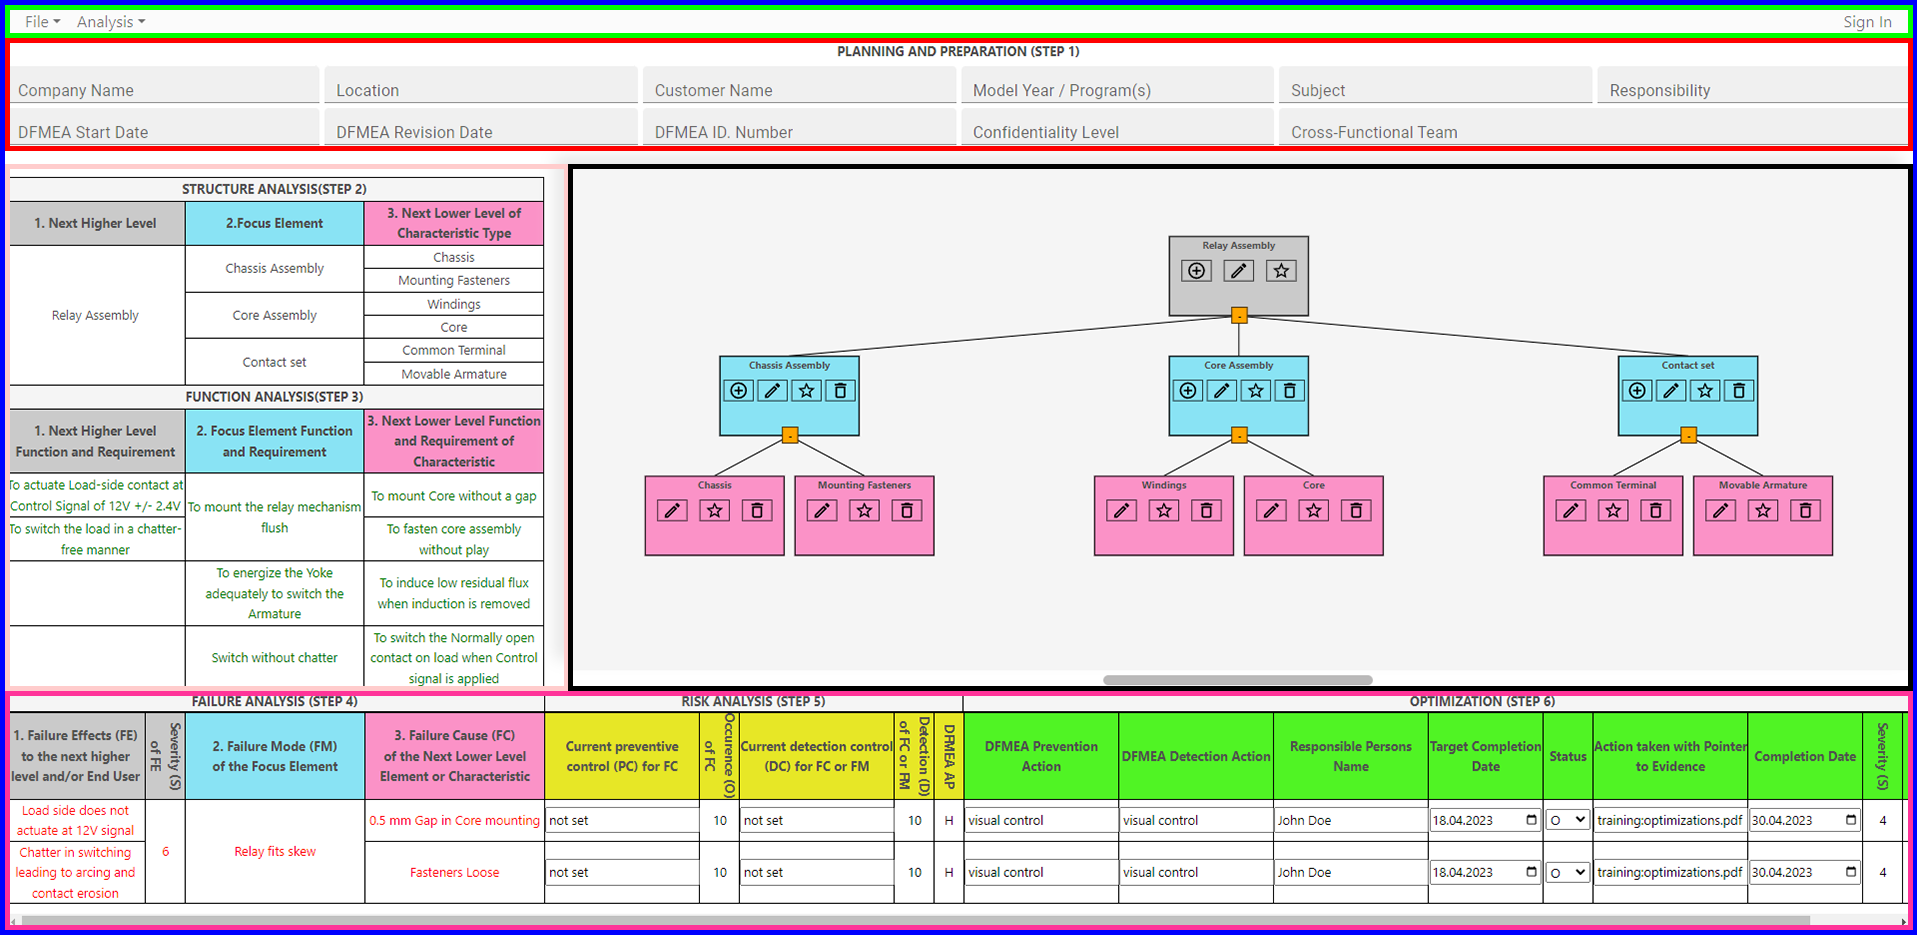
\includegraphics[width=1.0\textwidth]{Figures/componenty2P.png}
	\caption{Struktura aplikace}
	\label{fig:structure}
\end{figure}

\begin{itemize}
    \item Poslední důležitou komponentou je \textcolor{orange}{Modal}, která je zobrazena na obrázku \ref{fig:modal}. Modal umožňuje používat aplikaci jednoduše bez přecházení na jiné podstránky aplikace. Modal je tzv. modální okno, které se zobrazuje jakoby na nové vsrtvě stránky. Vyvolání zobrazení tohoto modálního okna je možné zpravidla kliknutím na tlačítko nebo položku v menu. Podle elementu, který vyvolal zobrazení modálního okna se zobrazí i odpovídající obsah. Modal může například sloužit pro úpravu objektů v rámci grafického náhledu, zobrazení tabulky pro hodnocení rizik, registrace a přihlášení k uživatelskému účtu apod. Zavření modálního okna je provedeno kliknutím kdekoli mimo okno nebo stisknutí klávesy Escape. 
\end{itemize}
\begin{figure}[t]
\centering
	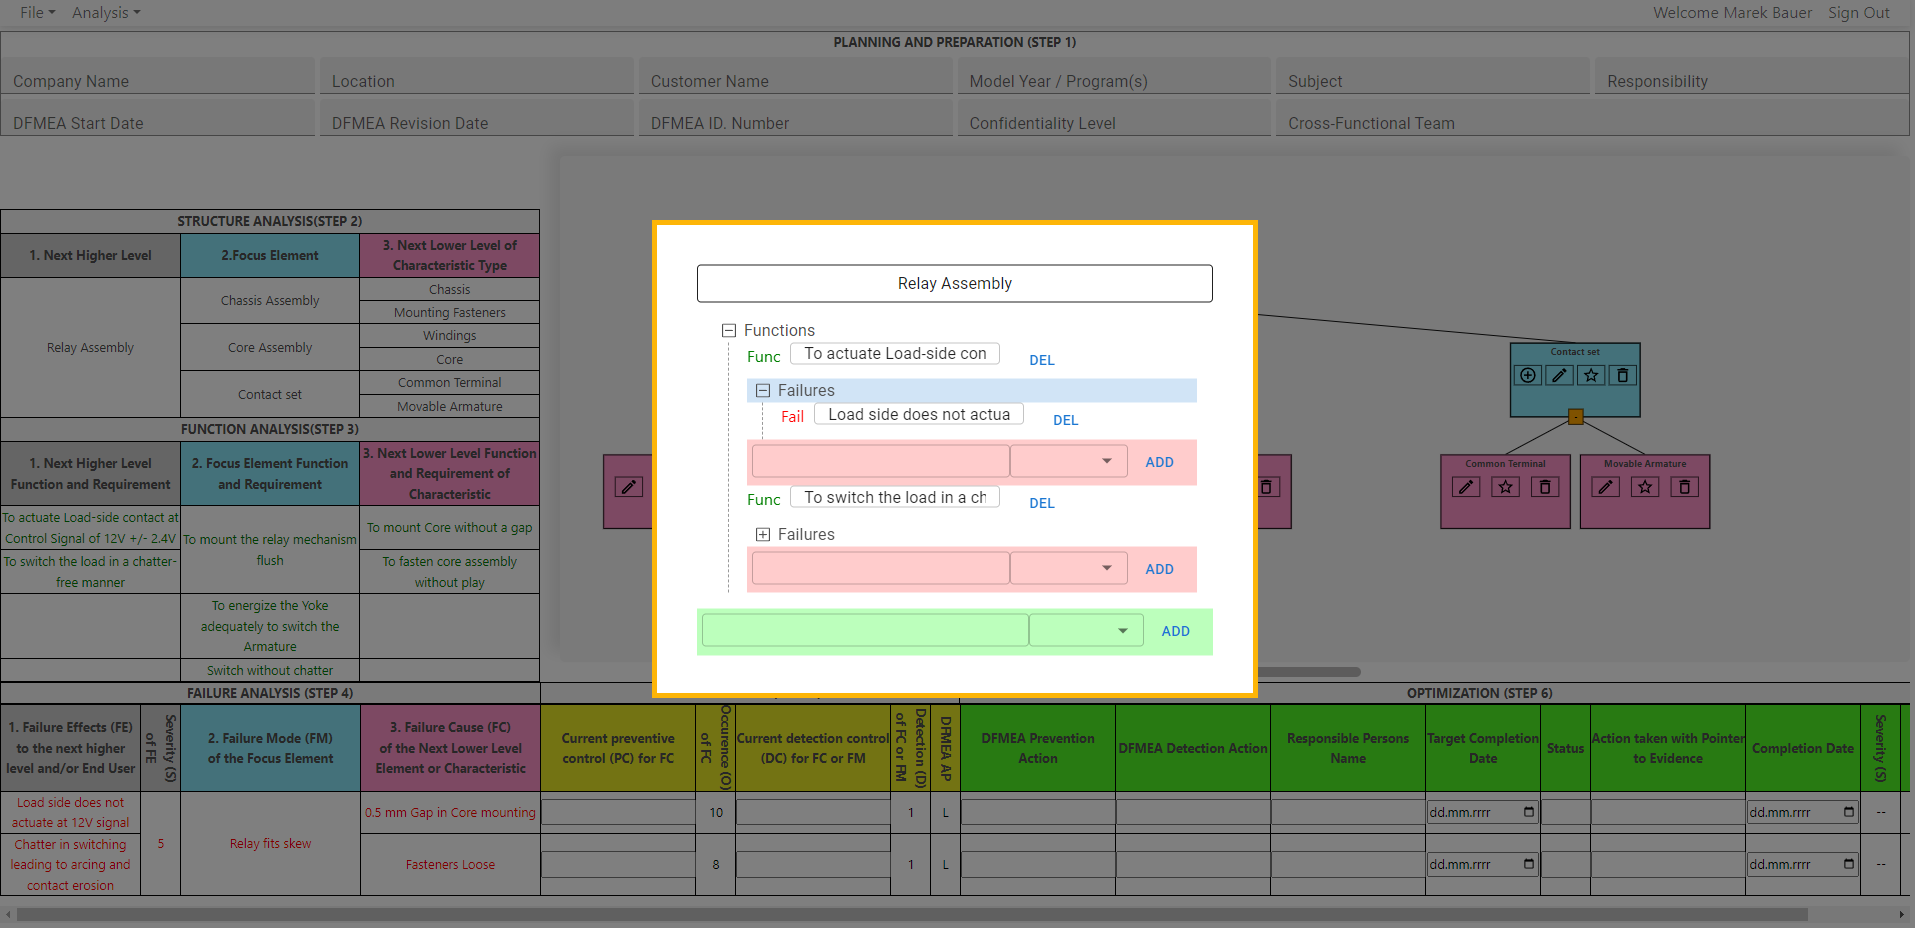
\includegraphics[width=1.0\textwidth]{Figures/modalP.png}
	\caption{Modální okno(komponenta)}
	\label{fig:modal}
\end{figure}

\newpage
\subsection{Tvorba analýzy}
Začátek tvorby analýzy se provádí vybráním typu analýzy zaměřené na návrh nebo proces. Na základě této volby se upráví několik několik hlaviček tabulky, které slouží pro detailnější popis toho, co se má vyplňovat. Dále se také upraví hodnotící tabulky, které obsahují slovní reprezentaci stupnice pro určení hodnotících atributů. Všech šest tabulek pro hodnocení se v rámci obou typů liší a to jak obsahem, tak bohužel i počtem sloupců a strukturou. Z toho důvodu nebylo možné při implementaci uložit tyto data do stejné datové struktury a dále je jednotným způsobem zpracovat a zobrazit, ale bylo potřeba jednotlivé zobrazení a data vytvořit manuálně. 

Následuje první krok analýzy a to vyplňení hlavičky se základními údaji o analýze. V této části by bylo dobré zmínit knihovnu, která se využívá na několika místech v rámci webové aplikace. Jméno této knihovny je Material UI \cite{mui}, která nabízí použití předem vytvořených komponent zejména v rámci formulářů a dalších funkčních prvků. Příkladem jsou textové vstupy v hlavičce dokumentu. Tyto textové vstupy jsou komponenty TextField importované z této knihovny s nastavením vlastních parametrů pro určení názvu, funkce zpracovávající události a také výběr z předem definových stylů. Další podstatné komponenty, které jsou použity v aplikaci: 
\begin{itemize}
    \item \textbf{Box} - Komponenta, která slouží jako zapouzdřující element obsahující další prvky. Obdoba HTML elementu div.
    \item \textbf{Modal} - Modal je komponenta popsaná již v předchozí kapitole zaměřené na popis struktury z pohledu komponent. Důležitou součástí této komponenty jsou parametry open a onClose, kterým je potřeba nastavit proměnnou a funkci, které určují, kdy je modal viditelný a jaká funkce se provede po vyvolání události pro zavření modalního okna.  
    \item \textbf{Button} - Tlačítko s předem daným stylem. Lze nastavit typ, variantu, formulář a metodu pro zpracování události při kliknutí. 
    \item \textbf{Treeview} - Tato komponenta je využita v rámci úpravy objektů v grafickém náhledu a slouží pro zobrazení stromové struktury funkcí a selhání podobně jako při zobrazení adresářové struktury v počítači. V rámci parametrů komponenty lze nastavit i vlastní ikony, které slouží pro rozbalení nebo zabalení odpovídajících položek. Jednotlivé položky v rámci stromové struktury jsou vlastně další komponenty z knihovny MaterialUI a to StyledTreeItem.
    \item \textbf{Autocomplete} - Tato komponenta slouží jako vstup ve formuláři, která obsahuje seznam položek, ze kterých je možné vybrat. Tento seznam je definován jako pole v rámci parametru komponenty. Konkrétně se používá při určování relací mezi funkcemi a selháními, kdy pro nově vytvářené funkce nebo selhání na první a třetí úrovni, je potřeba vybrat vybrat funkci nebo selhání z druhé úrovně. Obdobou je kombinace HTML elementů select a option. 
    \item \textbf{List} - List je komponenta sloužící pro jednoduché zobrazení seznamu položek. Obsahuje další pomocné komponenty pro definování hlavičky, položky seznamu, tlačítka a ikony. Je použita v rámci zobrazení a výběru uložených analýz uživatelem. 
    \item \textbf{Tabs} - Poslední uvedená komponenta slouží pro členění obsahu do přepínatelných záložek s různým obsahem. Obsahuje další komponenty Tab a TabPanel pro definování záložky a obsahu, který se má zobrazit při kliknutí na záložku. Je využita v rámci definování vlastních příkladů pro určování hodnotících atributů (Vážnost, Výskyt, Detekce) na počátku analýzy. 
\end{itemize}

Kromě těchto komponent je z knihovny použito několik volně dostupných ikon, které se vyskytují, jak součást komponent, tak samotně například pro vzhled tlačítek v rámci objektů v grafickém režimu. Tvorba analýzy dále pokračuje v rámci grafického a tabulkového náhledu na analýzu, který bude popsán v rámci samostatných kapitol.  

\subsubsection{Grafický náhled na analýzu}
\label{sec:grafika}
Grafický náhled slouží zároveň i pro tvorbu analýzy pro kroky: analýza struktury, funkcí a selhání. Náhled zajišťuje dříve zmíněná komponenta TreeGraph. Pro zobrazení stromové struktury objektů je použita knihovna React D3 Tree \cite{d3tree}. Tato knihovna je nadstavbou obsáhlé knihovny D3.js, která umožňuje zobrazení a manipulaci s grafickými objekty pomocí Javascriptu. Použitá knihovna umožňuje zobrazení stromové struktury objektů tím, že se v rámci importované komponenty Tree definuje jako parametr data, objekt s atributem children, což je pole dalších objektů na další úrovni stromu. Knihovna implicitně poskytuje některé funkce pro práci s tímto grafickým zobrazením jako je přibližování a oddalování zobrazeného obsahu, posouvání struktury tažením myší, zobrazení a skrytí prvků na další úrovní apod. Dále je také možné použít vlastní implementaci pro některé části řešení. Příkladem je nastavení vlastních čár spojující jednotlivé objekty nastavení parametru komponenty pathFunc nebo použití vlastních tvarů a obsahu jednotlivých objektů nastavením parametru renderCustomNodeElement.

Obě tyto možnosti byly při implementaci využity. První funkci bylo potřeba nastavit svg objekt, který znázorňuje přímku s počátečními a koncovými souřadnicemi x a y podle šířky objektu. Druhá možnost nastavení vlastních tvarů a obsahu objektů byla vyřešena vytvořením vlastních komponent, které obsahují jednak definovaný tvar, ale také název objektu a sadu nástrojů pro manipulaci s objekty. Detailní ukázku této komponenty je možné vidět na obrázku \ref{fig:node}. Komponeta obsahuje(seznam nástrojů je popsán z levé strany): 


\begin{figure}[h]
\centering
	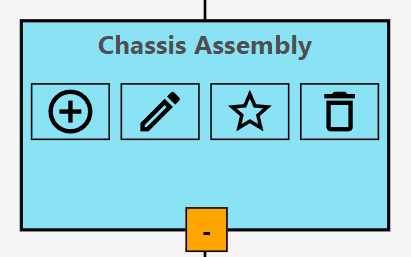
\includegraphics[width=0.7\textwidth]{Figures/node.png}
	\caption{Komponenta objektu v grafickém režimu}
	\label{fig:node}
\end{figure}


\begin{itemize}
    \item \textbf{Jméno objektu} - Název objektu v rámci stromové struktury. 
    \item \textbf{Přidat} - Pomocí tohoto tlačítka se přidává danému objektu další potomek. 
    \item \textbf{Upravit} - Toto tlačítko slouží pro zobrazení modálního okna, kde lze nastavit jméno objektu. Dále přidávat, editovat a mazat funkce a selhání, které odpovídají danému objektu ze strukturální analýzy. Objekt vždy obsahuje seznam funkcí a k tomu odpovídající seznam selhání, které je možné zobrazit nebo skrýt. Na konci těchto seznamů je vždy formulář, který slouží pro přidání nové funkce nebo selhání. Všechny zobrazené hodnoty jsou zobrazeny v textovém vstupu a jejich hodnota lze kdykoli upravit. Ukázka této funkce již bylo možné zhlédnout při popisu komponenty Modal na obrázku \ref{fig:modal}.
    \item \textbf{Označit} - Tlačítko, které nabízí jednu z dalších zajímavých funkcí aplikace. Pomocí kliknutí na toto tlačítko se označí objekt a všechny jeho přidružené funkce a selhání, reprezentované buňkami v tabulkovém zobrazení, oranžovou barvou. Díky tomu je v tabulce jednoznačně možné určit, které hodnoty mezi sebou navzájem souvisí. Tato funkce byla implementována jednoduchým polem identifikátorů, které se kontrolují při renderování tabulky. 
    \item \textbf{Smazat} - Poslední tlačítko v sadě nástrojů slouží pro odstranění objektu ze struktury. Úskalím při implementaci bylo tzv. kaskádové mazání. Při smazání objektu v rámci struktury je potřeba také smazat všechny jeho přidružené funkce a selhání, které se navíc v rámci zanořeného objektu vyskytují na více místech. 
    \item \textbf{Rozbalit/zabalit} - Poslední tlačítko již není v seznamu nástrojů, ale nachází se na spodní straně objektu. Slouží pro zobrazení nebo skrytí potomků daného objektu. 
\end{itemize}

K popisu těchto komponent ještě patří pravidlo, že kořenový objekt neobsahuje možnost pro jeho smazání a objekty na třetí úrovní neobsahují možnost pro přidávání dalších potomků. Je to z důvodu dané logiky strukturální analýzy. 

Jedno z implementačních rozhodnutí se týkalo volby orientace stromové struktury. Knihovna nabízí obě varianty, tedy zobrazení horizontální i vertikální. Nakonec bylo vybráno zobrazení horizontální z důvodu toho, že se struktura při tvorbě rozsrůstá spíše do šířky než do výšky a vzhledem k tomu jaké má komponenta pro grafické zobrazení míry, tak se toto rozhodnutí zdálo přívětivější. 


\subsubsection{Tabulkový náhled na analýzu}
Zobrazení analýzy pomocí textové tabulky je druhá varianta, která slouží pro tvorbu analýzy. Oproti grafickému režimu pak slouží k tvorbě analýzy rizik a případně stanovení optimalizačních opatření. Z implementačního pohledu bylo zobrazení některých dat docela náročné z důvodu správného zobrazení relací mezi atributy a odpovídajícího slučování buněk. Tabulkám bylo potřeba nastavit fixní layout a určit přímo šířku všech sloupců, aby tabulka neměnila velikost při zadávání různě dlouhého obsahu. V tabulkovém zobrazení se hodně pracuje s hlavním objektem, ve kterém jsou uložena všechna potřebná data. Běžný problém, který se řeší ve webových aplikací je to, aby měly všechny potřebné komponenty přístup ke stejným datům. Řešením tohoto problému je použití knihovny React-redux \cite{redux} , která slouží jako globální stav nějakých dat a umožňuje komponentám přístup k tomuto stavu a jeho modifikaci. Stavy se skládají z těchto čtyř souborů: 
\begin{itemize}
    \item \textbf{Reducer} - Hlavní soubor, který obsahuje inicializaci objektu s atributy, který slouží pro určení nějakého stavu. Dále obsahuje metodu, jejímiž atributy jsou state a action. Akce je objekt skládající se z parametrů type a payload. Na základě typu akce se pak provede příslušná modifikace stavu. V případě této knihovny je nutné vždy vracet nový objekt a ne pouze modifikovat aktuální. 
    \item \textbf{Typy} - Tento pomocný soubor obsahuje výčet všech typů akcí, které mohou v rámci daného stavu nastat. 
 \item \textbf{Akce} - Zde jsou obsaženy všechny akce, které mají komponenty k dispozici pro práci s daným stavem dat. V rámci komponent je potřeba použít speciální metodu \textit{useDispatch}, která vrací objekt umožňující vyvolání nějaké akce. Tyto akce pak zachytává a zpracovává reducer. 
 \item \textbf{Selektor} - Poslední soubor se používá se pro získání stavu dat. Selektor může obsahovat metody, které uložené data nějakým způsobem filtrují nebo modifikují a vrací požadovanou strukturu. 
\end{itemize}
V rámci zobrazení tabulky se používájí metody v rámci selektoru, které filtruje zejména definové funkce a selhání v rámci analýzy z hlavního objektu do pole. Pomocí tohoto pole je pak snažší zobrazit požadované relace při renderování buněk tabulky. 

Co se týká tvorby samotné tabulky tak je potřeba vyfiltrované data zobrazit odpovídajícím způsobem tak, aby byly dodrženy všchechny požadované relace. Pro průchod daty jsou použity cykly, které postupně tvoří textový řetězec, který je následně převeden do reprezentace HTML elementů. Horizontální tabulka také obsahuje sadu formulářových vstupů jako je tlačítko pro zobrazení modálního okna, textový vstup, výběr ze seznamu nebo výběr datumu.


\subsubsection{Podpůrné funkce}
Tyto funkce slouží pro zjednodušení tvorby analýzy tím, že poskytují nastavení vstupních hodnot, zaznamenávaní aktivit při setkání týmu a výstup z analýzy. Zde je seznam těchto funkcí a jejich krátky popis:
\begin{itemize}
    \item \textbf{Nastavení vlastních příkladů pro určení hodnotících atributů} - Tato funkce slouží pro nastavení clastních příkladů v rámci atributů Vážnost, Výskyt a Detekce. Tato činnost by se měla provést před začátkem vypracování samotné analýzy. Nastavení se provádí v rámci modálního okna, které obsahuje pro všechny tři atributy deset textových vstupů, kde je možné definovat slovní hodnocení rizik. Toto hodnocení se pak zobrazuje v příslušných tabulkách hodnotících atributů. 
    \item \textbf{Tvorba zápisu ze setkání týmu} - Další funkce slouží pro zaznamenávání aktivit z jednotlivých sektání týmu. Jedná se vlastně o tabulku s atributy: ID, Datum, Popis, Související dokumenty a Aktualizováno. Zápisy jsou zobrazeny v tabulce, pod kterou se nachází formulář pro přidání nového zápisu. 
 \item \textbf{Kontrola úplnosti analýzy a výsledky} - Tato funkce slouží zejména pro závěrečnou fázi analýzy. Jak je vidět na obrázku \ref{fig:results}, tak funkce zobrazí graf obsahující rozdělení všech rizik do tří hodnot AP(Low, Medium, High), zároveň jsou rizika dělena na počáteční a koncová. Na základě těchto dvou hodnot je také možné zobrazené slouce filtrovat, kliknutím na popis dané hodnoty na horní straně grafu. Tato i všechny ostatní funkce jsou součástí knihovny Chart.js \cite{chart}, která byla použita pro zobrazení grafu. 
 Pod grafem se nachází tabulka, která ve zjednodušeé formě obsahuje všechna nalezená rizika. Zároveň je zde kontrola, že všechny rizika jsou v jednom z konečných stavů, tedy optimalizována nebo určena, že není potřeba optimalizovat. Stav pro určení rizika, které nepotřebuje optimalizaci lze určit kliknutím na políčko v tabulce. Změna tohoto stavu má za následek, že i zbytek řádku tabulky pro optimalizaci daného rizika je znepřístupněn a nelze psát do formulářových vstupů hodnoty. 
\end{itemize}

Na závěr popisu tvorby analýzy je ještě dobré dodat, že aplikace na několika místech obsahuje informační vysvětlivky. Příkladem je práce s objekty v grafickém režimu. Pro práci s objekty se používají tlačítka s ikonami, které při najetí myši zobrazí krátkou vysvětlivku o činnosti daného tlačítka. Druhým příkladem je zobrazení dodatečné informace při najetí na hodnotu AP v rámci tabulkového náhledu. V tomto případě se zobrazí informace o hodnotě RPN na základě, které byla určena hodnota AP. 
\begin{figure}[h]
\centering
	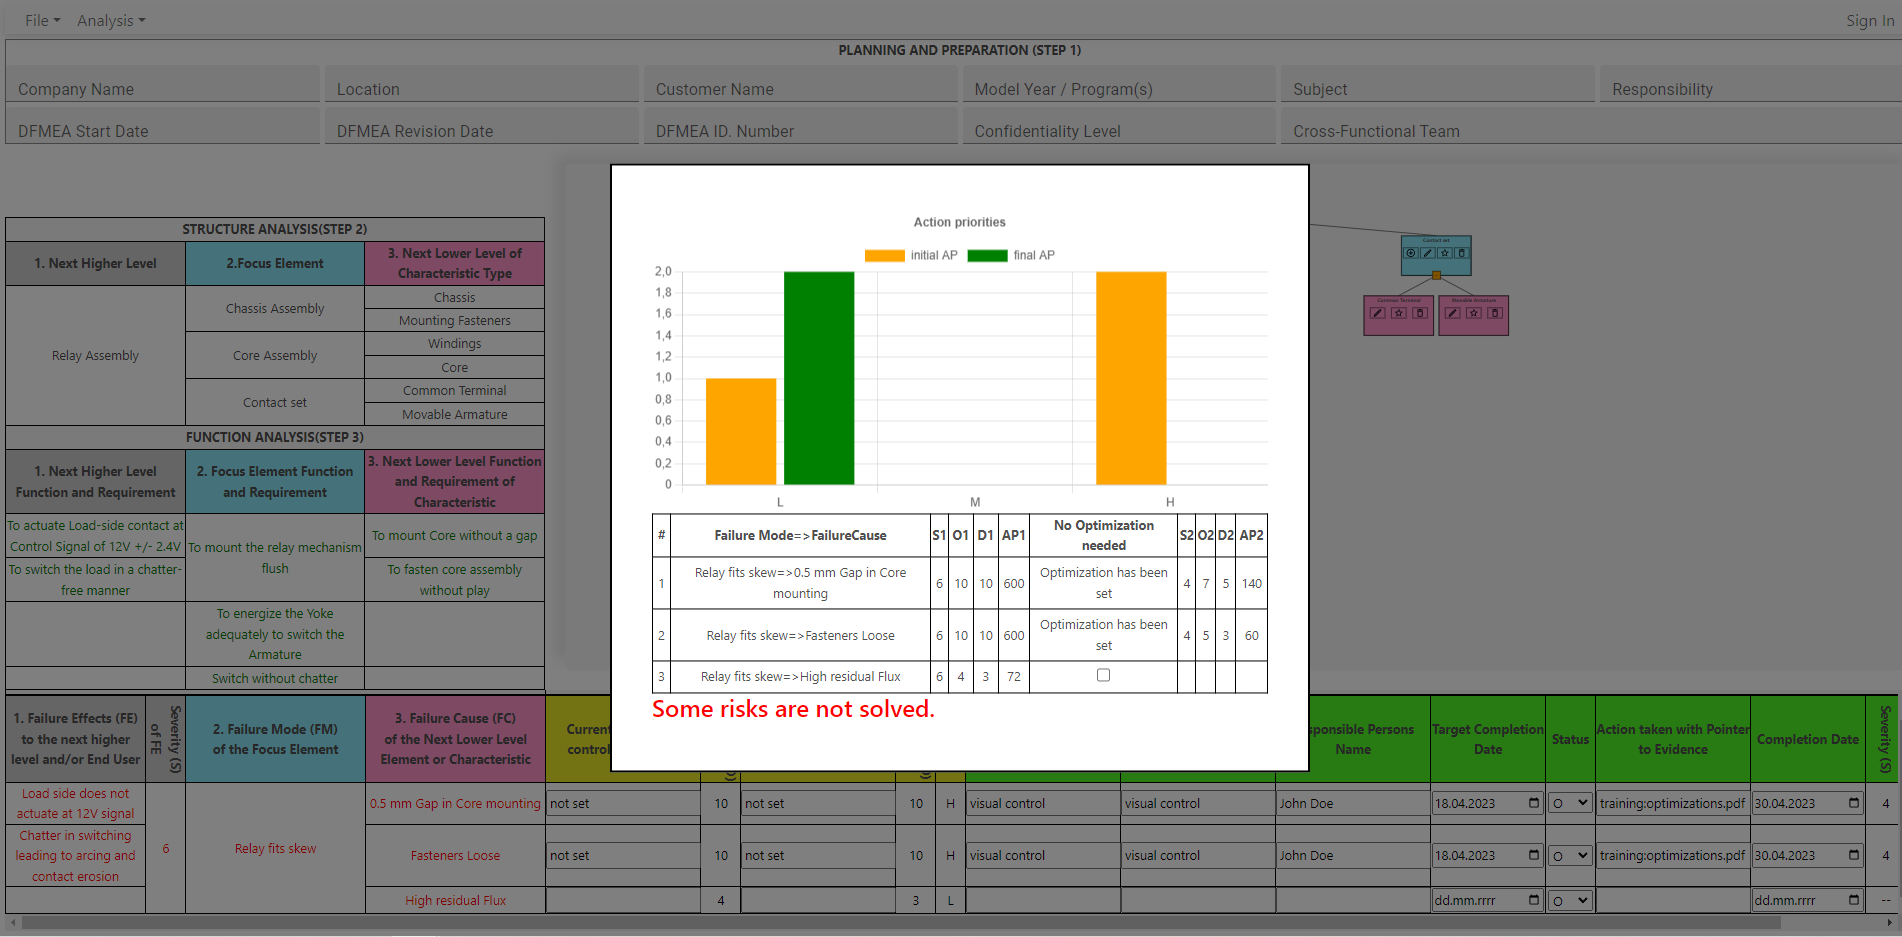
\includegraphics[width=1.0\textwidth]{Figures/results.png}
	\caption{Zobrazení výsledků analýzy}
	\label{fig:results}
\end{figure}

\newpage
\subsection{Správa uživatelkých účtů}
Nástroj nabízí základní možnosti pro přihlášení k uživatelskému účtu. Účet slouží pro zpřístupnění funkcí pro ukládání a načítaní analýzy z databáze. Formulář pro přihlašování je také vyřešen pomocí modálního okna(obr. \ref{fig:sign}). Možnosti přihlášení jsou dvě: 
\begin{itemize}
    \item \textbf{Pomocí vlastního účtu} - Pomocí této možnosti je nutné se nejdříve registrovat zadáním uživatelského jména, emailu a hesla.  
    \item \textbf{Pomocí Google účtu} - Druhá možnost nabízí přihlášení k účtu uživatelskému účtu pomocí již vytvořeného účtu v rámci aplikace Google.
\end{itemize}

\begin{figure}[t]
\centering
	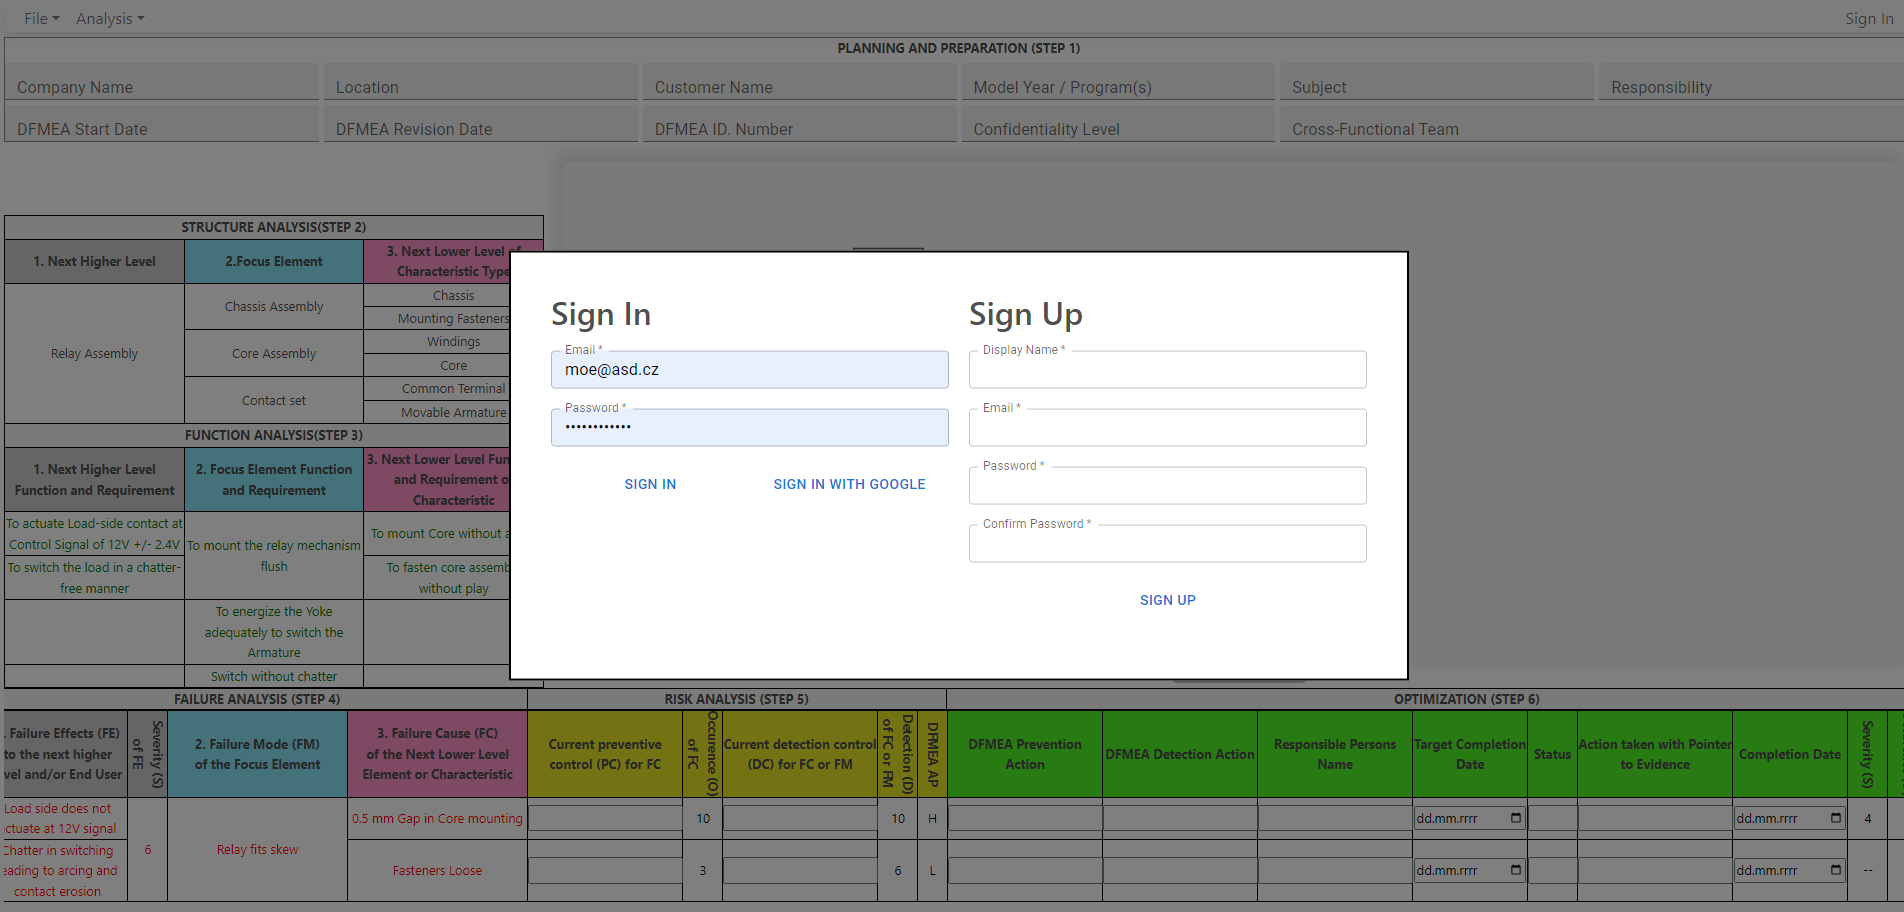
\includegraphics[width=1.0\textwidth]{Figures/sign.png}
	\caption{Přihlašování k uživatelskému účtu}
	\label{fig:sign}
\end{figure}

Obě tyto možnosti poskytuje platforma pro vývoj webových aplikací Firebase \cite{firebase}. Po založení vlastního účtu na této platformě je možné využít jejich nástroj k autentizaci, kde lze povolit přihlašování pomocí různých možností. Platforma poskytuje vlastní API, pomocí kterého lze využívat metody při implementaci. Prvním krokem je incializace aplikace pomocí konfigurančních údajů, které jsou součástí účtu. Dále lze využít například metody \textit{singInWithGooglePopup}, která slouží pro vyvolání pop-up okna s možností přihlášení ke Google účtu. Další velice zajímavou nabízenou funkcí je poskytnutí metody, která funguje na principu návrhového vzoru observer. V kombinaci s ukládáním stavu o uživateli pomocí React-redux knihovny lze reagovat na změny stavu o přihlášeném uživateli. 

V rámci správy uživatelů je také vytvořena jednoduchá funkce pomocí, které lze automaticky kopírovat odkaz na aktuální analýzu do schránky. Odkaz má tento formát: doména/analyses/\uv{unikátníID}. O zkopírování adresy do schránky je uživatel informován jednoduchým pop-up oknem, který vystupuje v aplikaci jako samotatná komponenta a může být využita pro sdělení různých krátkých informací.  


\subsection{Export a import}
Poslední uvedenou funkcí nástroje je export a import částí analýzy do různých formátů. V rámci této funkce si tak může uživatel načítat a ukládat data jako soubory na své zařízení. Základní funkcí je export a import dat analýzy do formátu JSON. Díky této možnosti si může uživatel uložit stav své analýzy do tohoto souboru a kdykoliv jej načíst zpět. Při importu dat ze souboru se provádí základní ověření správnosti formátu. Konkrétně je v aplikaci vytvořena datová struktura Map, která má formát klíč-hodnota. Klíčem jsou všechny atributy, které může objekt obsahovat a hodnota je jejich datový typ. Pokud má importovaný objekt atributy, které neodpovídají dané mapě, tak není objekt importován. 

V rámci grafického režimu je vytvořena stromová struktura, kterou lze také exportovat do formátu PNG. Pro vytvoření tohoto obrázku bylo potřeba modifikovat danou strukturu, tak aby zbytečně neobsahovala nástroje pro modifikaci objektů. Zde je také vidět výhoda komponent a to jejich znovupoužitelnost. V aplikaci se tak vyskytuje komponenta s grafem ve dvou verzích, kdy jedna obasahuje objekty s upraveným vzhledem pro export. Obsah této komponety je pak stáhnut pomocí balíčku react-component-export-image \cite{exportIMG}. Výsledek je možné vidět na obrázku \ref{fig:graphPNG}.

\begin{figure}[h]
\centering
	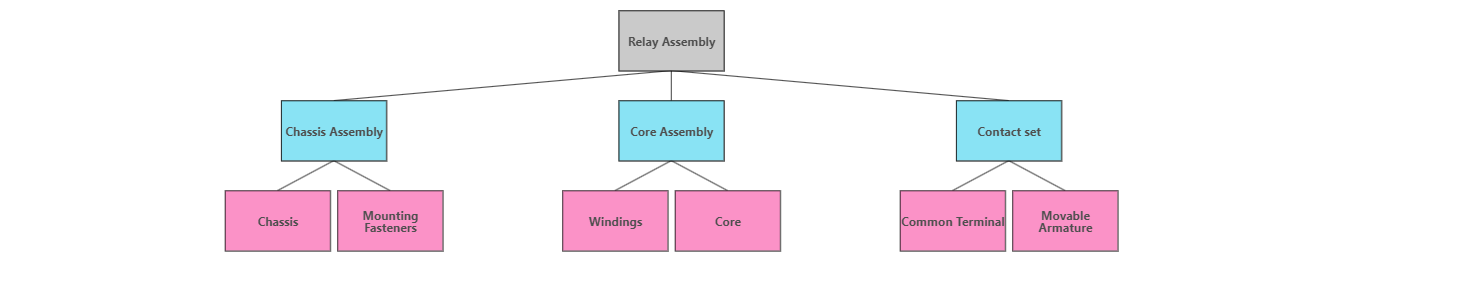
\includegraphics[width=1.0\textwidth]{Figures/Relay_Assembly.png}
	\caption{Export struktury do formátu PNG}
	\label{fig:graphPNG}
\end{figure}

Poslední funkcí pro export je možnost stáhnout celý tabulkový náhled na analýzu do formátu XLS, který lze otevřít například pomocí tabulkového editoru Microsoft Excell. Pro tuto funkci byl použit balíček react-export-table-to-excel \cite{exportTable}, který obsahuje metodu pro export dokonce více tabelkových elementů, které jsou v rámci jednoho obalujícího elementu. Problém při použití této nebo jiné knihovny, že i zde bylo potřeba upravit tabulku pro export. Jednak musela být použit složitější způsob renderování tabulky a slučování buněk a také v některých částí tabulky bylo potřeba nahradit prvky formulářů jejich hodnotami. Toho bylo docíleno rekurzivní funkcí, která postupně procházela potomky tabulkového elementu a při nálezu formulářového vstupu je nahradila jejich hodnotou. Výstřižek ze zobrazení pomocí tabulkového editoru je vidět na obráku  \ref{fig:excel} . 

\begin{figure}[h]
\centering
	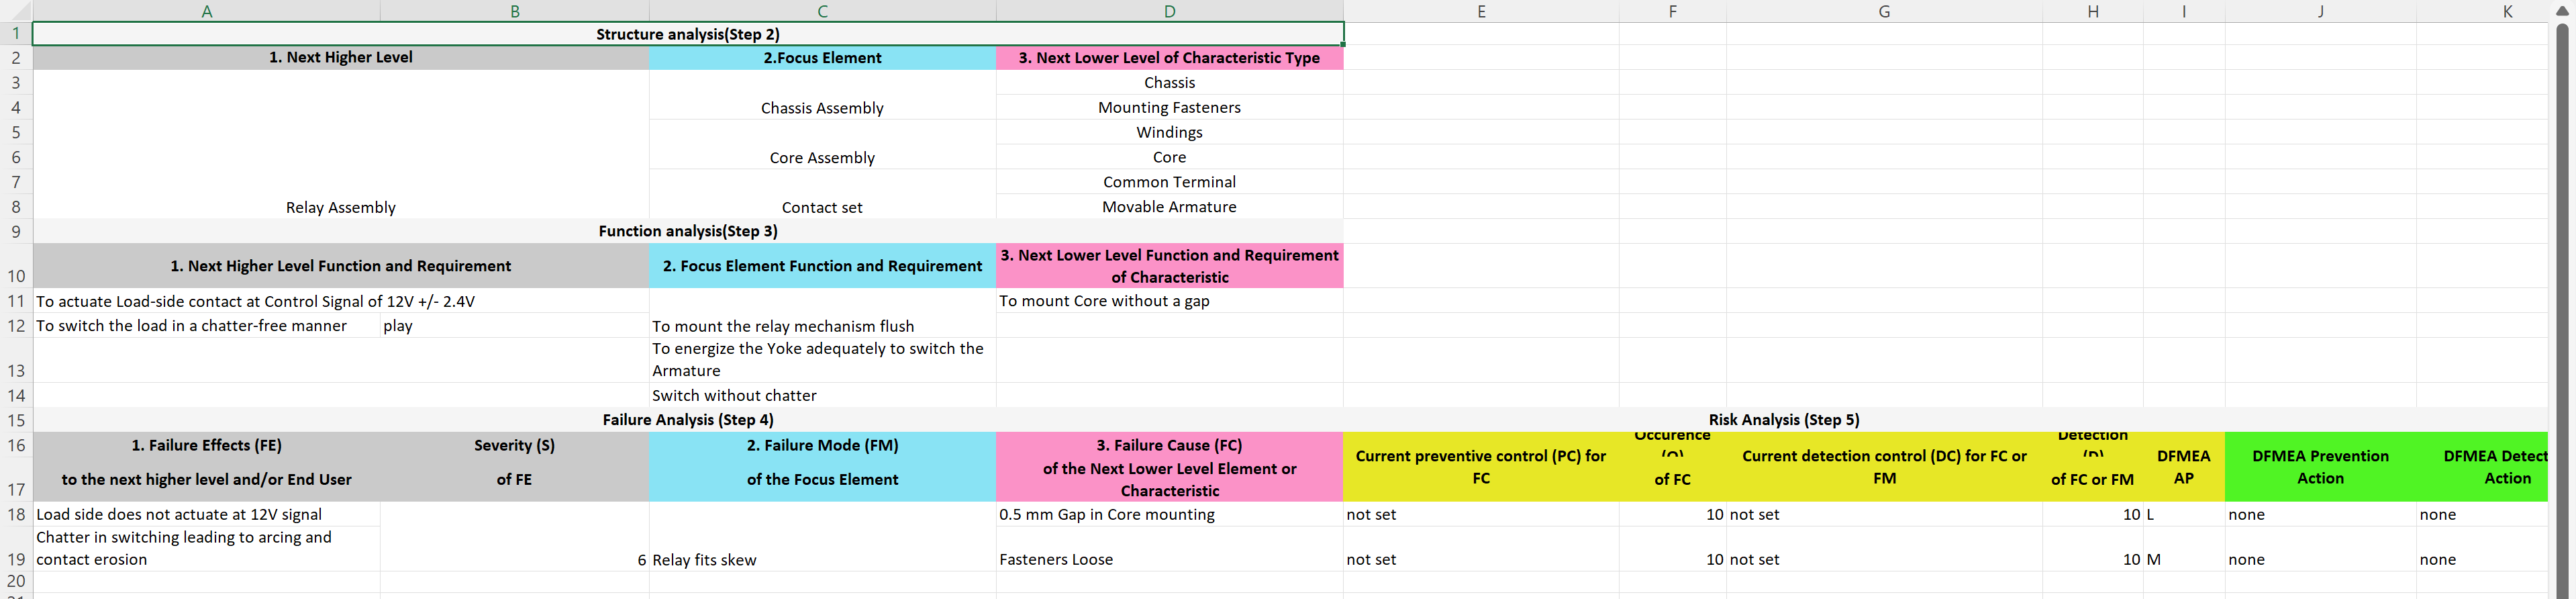
\includegraphics[width=1.0\textwidth]{Figures/excel.png}
	\caption{Export tabulky do formátu XLS}
	\label{fig:excel}
\end{figure}

Výhodou těchto exportů je, že si uživatel může dodatečně upravit a přípapdně vytisknout jednotlivé části analýzy. U všech těchto exportů je nastavno jméno souboru podle kořenového objektu v rámci analýzy struktury. 

\section{Testování}
Pro testování aplikace byly zvoleny systémové testy, nebo-li testy, které mají za cíl ověřit funkčnost jednotlivých případů užití. Systémové testování se provádí jako jedno z posledních před samotným nasazením aplikace do produkce. Pro toto testování se v praxi využívají dva způsoby. První způsob je projít jednotlivé scénáře manuálně se snahou nalézt případné nedokonalosti. Druhý způsob je použití automatizovaných testů, které simulují chování uživatele. V rámci této diplomové práce byl nakonec zvolen způsob manuálního otestování aplikace dvěma nezávislými osobami. Důvodů pro toto rozhodnutí je více. Například v praxi by měl být tento způsob testování bežnější. Automatizované testy jsou v tomto případě zbytečně nákladné a ne tolik efektivní a hodí se spíše provádět automatizované testování komponent nebo integrační testy, které ověřují správnou provázanost komponent. Proto jsou ve firmách lidé, kteří procházejí jednotlivé případy užití samostatně a vytvoří zprávu, kde zhodnotí daný průchod scénářem. Další výhodou tohoto přístupu je, že test provádí jiná osoba než ta, která vytvořila danou aplikaci. V případě psaní testu vývojařem může dojít k přehlednutí akcí, které by jiný uživatel udělal jinak. 

Pro testování nástroje pro tvorbu FMEA byly osloveni dva kolegové, kterým byl dán přístup k produkční verzi aplikace pomocí repozitáře na GitHubu. O jednoduché spuštění aplikace pomocí jednoho příkazu se stará program Docker. Popis instalace nástroje je součástí přílohy \ref{sec:docker}. Dále byly vytvořeny tři případy užití, které pokrývají značnou část funkcionality nástroje. Tyto případy užití jsou součástí přílohy \ref{sec:UC}. Pro hodnocení testů byl také vytvořen jednoduchý formulář obsahující otázky ke každému testovacímu případu. 

\subsection{Zhodnocení provedených testů}
Formulář, který měli oslovení kolegové vyplňovat se skládal z otázky, jestli se podařilo naplnit účel v rámci každého případu užití. Dále také měli možnost vyplňit vlasními slovy připomínky, nedokonalosti, návrhy na zlepšení, na které při provádění daného testu narazily. Shrnutí těchto odpovědí jsou zobrazeny v tabulce \ref{tab:testovani}. 

Jak je vidět tak se podařilo projít všemi testovacími případy bez větších potíží. Některé připomínky pramenily z nekompletních znalostí problematiky FMEA, které by v praxi neměli být velkým problémem, kdy se počítá, že bude tým provádějící analýzu dostatečně obeznámem s jejími aspekty. Nicméně připomínky pro zpřehlednění a úpravu některých částí UI byly brány v potaz a třeba v případě vyplňování atributu Status byl nahrazen textový vstup výběrem možností ze seznamu. Většina nalezených problémů byla také dodatečně opravena. 

Toto testování mělo za cíl zjistit, jestli byl zvolen správný přístup při návrhu aplikace, tak aby uživatel přistupující k aplikaci, dokázal provádět zadané úkony. Jednotlivé případy užití byly definovány obecně bez konkrétních zadání na, co by měl uživatel kliknout apod. I přes to se těmto dvěma uživatelům bez hlubších znalostí dané problematiky podařilo projít danými případy bez větších potíží. Dalším cílem bylo také objevit možné nedokonalosti a chyby, které se vyskytly při procházení jinými subjekty.  


\begin{table}[h]
	\caption{Výskedky testování}
	\label{tab:testovani}
\begin{tabular}{|p{3cm} | p{6cm} | p{6cm} |}
\hline
 & \textbf{Tester \#1} & \textbf{Tester \#2} \\ \hline
 \multicolumn{3}{|c|}{\textbf{UC1: Tvorba FMEA}} \\\hline
\textbf{Podařilo se \break naplnit účel}? & ANO & ANO\\ \hline
\textbf{Připomínky} & Lepší popis prvků UI v grafickém režimu(label, placeholder,...). & Více prostoru pro zobrazení textu v rámci tabulkového režimu(např. atribut Status). \\ \hline
 \multicolumn{3}{|c|}{\textbf{UC2: Přihlášení k uživatelskému účtu}} \\\hline
\textbf{Podařilo se \break naplnit účel}? & ANO & ANO\\ \hline
\textbf{Připomínky} & Zlepšit validační hlášky při registraci.  &  \\ \hline

 \multicolumn{3}{|c|}{\textbf{UC3: Ukládán\&Načítání analýzy}} \\\hline
\textbf{Podařilo se \break naplnit účel}? & ANO & ANO\\ \hline
\textbf{Připomínky} & 
\begin{enumerate}

    \item  Občasné problémy s uložením nové analýzy.(Krok č.1)
    \item  Při přepnutí uživatelského účtu by se mohla vytvořit nová analýza.
    \item  Přidat možnost pojmenování analýzy při ukládání.
    \item  Problém s importem analýzy ze souboru v kombinaci s načtením analýzy z databáze.

\end{enumerate}
  &  
  
  \begin{enumerate}
    \item  Ukládání pouze pomocí jednoho tlačíka, které buď vytvoří nový záznam analýzy nebo uloží aktualizuje již uložený.
    \item  Zlepšit popis okna pro načítání analýz. (například pomocí tabulky s atributy)

\end{enumerate} 
\\ \hline

\end{tabular}\  
\end{table}


%\chapter{Testovaní}
\label{sec:testovani}
\begin{longtable}{p{4cm} | p{12cm} } 
        \caption{UC1:Tvorba FMEA}
\label{tab:compare}
\\
Název & UC1:Tvorba FMEA \\ \hline
Účel &  \\  \hline
 &  \\ \hline
 &  \\ \hline
 &  \\ \hline
 &  \\ \hline
 &  \\ \hline
 &  \\ \hline
 &  \\ \hline
 &  \\ \hline
 &  \\ \hline
 &  \\ \hline
 &  \\ \hline
 &  \\ \hline
\end{longtable}

\begin{table}[h]
	\caption{UC2: Export\&Import analýzy}
	\label{tab:uc2}
\begin{tabular}{p{4cm} | p{12cm} }
Název & UC2: Export\&Import analýzy \\ \hline
Účel &   Exportování analýzy do formátů JSON, XLS, PNG a import z formátu JSON. \\\hline
Hlavní aktér  & Uživatel  \\ \hline
Prekondice & Uživatel se nachází na hlavní stránce aplikace \\ \hline

        Základní scénář &  \begin{enumerate}
     \item Uživatel zvolí akci pro exportování analýzy do formátu JSON.
     \item Systém převede data analýzy do formátu JSON a otevře okno pro uložení souboru na disk.
     \item Uživatel zvolí akci pro exportování struktury analýzy do formátu PNG.
     \item Systém provede úpravu struktury a zobrazí okno pro uložení souboru na disk. 
     \item Uživatel zvolí akci pro exportování tabulky analýzy do formátu XLS.
     \item Systém provede sloučení tabulek a zobrazí okno pro uložení souboru na disk. 
     \item Uživatel zvolí akci pro import analýzy z formátu JSON.
     \item Systém zobrazí okno pro vybraní souboru z disku. 
     \item Uživatel vybere soubor z disku. 
     \item Systém převede data z JSON formátu a provede validaci vybraného souboru. 
     \item Systém načte data analýzy.
     
     
\end{enumerate}\\ \hline
Alternativní scénář  &  
\begin{itemize}
    \item [11.1] Systém zobrazí informaci o chybném formátu vybraného souboru. 
\end{itemize}
\\ \hline
Realizované požadavky\\ \hline
\end{tabular}\  
\end{table}
\chapter{Závěr}
\label{sec:zaver}
asasdads 

%\input{Chapters/Introduction.tex}
%\input{Chapters/SampleChapter1.tex}
%\input{Chapters/SampleChapter2.tex}
%\input{Chapters/TechnicalDetails.tex}
%\input{Chapters/Conclusion.tex}


% Seznam literatury
\printbibliography[title={Literatura}, heading=bibintoc]

% Prilohy
\appendix
\chapter{Instalace webové aplikace}
\label{sec:docker}
Pro nasazení alikace je použit docker, což je software, který umožňuje běh aplikace v izolovaném prostředí tzv. kontejneru. Díky dockeru je možné spustit stáhnutý projekt použitím příkazu \uv{docker-compose up} v kořenovém adresáři projektu. Zde se nachází soubor s příponou yaml, který obsahuje skript pro vytvoření obrazu pro klientskou a serverovou část a spuštění aplikace na adrese: http://localhost:3000/. Pro otestování sdílení dat mezi uživateli je možné otevřít stránku se stejným url ve dvou separátních oknech. Díky většímu množství použitých knihovena a závislostí může prvotní instalace a spuštění trvat i několik minut. Docker konkrétně usnadňuje uživateli nutnost použití několika příkazů pro instalaci všech potřebných závislostí a spuštění serverové a klientské části. Tyto příkazy jsou obsaženy v souborech s názvem Dockerfile umístěných v adresářích /frontend a /backend. Standardně se řeší také inicializace a spuštění databáze. Nicméně toto bylo vyřešeno použitím cloudového řešení, ke kterému je možné se připojit z jakékoliv IP adresy. Běh aplikace v kontejneru je možné ukončit příkazem \uv{docker-compose down}.

\chapter{Případy užití pro testování}
\label{sec:UC}
\newpage

\begin{longtable}{p{4cm} | p{12cm} } 
     \caption{UC1: Tvorba FMEA}
        \label{tab:uc1}
\\
Název & UC1: Tvorba FMEA \\ \hline
Účel &   Tvorba FMEA pomocí šesti krokového postupu. \\\hline
Hlavní aktér  & Uživatel  \\ \hline
Prekondice & Uživatel se nachází na hlavní stránce aplikace. \\ \hline
Úspěšné dokončení & Uživatel prošel proces tvorby analýzy a uzavřel všechny nalezené rizika pomocí kontroly úplnosti analýzy. \\ \hline

        Základní scénář &  \begin{enumerate}
     \item Uživatel zvolí akci pro vytvoření nové analýzy(DFMEA/PFMEA).
     \item Systém inicializuje nová data se zvoleným typem analýzy.
     \item Uživatel vyplňuje atributy v rámci 1. kroku analýzy(Planning and preparation)
     \item Uživatel postupně vytváří strukturu produktu/procesu pomocí tlačítka uv{Add Node} pro jednotlivé objekty v rámci grafického náhledu na analýzu. (2. krok - Structure Analysis)
     \item Uživatel přidává funkce jednotlivým objektům strukturální analýzy pomocí tlačítka uv{Edit Node} (3. krok - Function Analysis)
     \item Uživatel přidává selhání jednotlivým funkcím pomocí tlačítka uv{Edit Node} (4. krok - Failure Analysis)
     \item Uživatel hodnotí nalezené selhání pomocí tabulkového náhledu na analýzu(5. krok - Risk Analysis). 
     \item Uživatel vyplňuje atributy pro optimalizaci aktuálních opatření \break (6. krok - Optimization). 
     \item Uživatel provede opětovné hodnocení rizika pomocí atributů(Severity, Occurance, Detection). 
     
\end{enumerate}\\ \hline

Alternativní scénář  &
\begin{itemize}
    \item [3.1] Uživatel zvolí možnost(Set SOD) pro určení vlastních příkladů pro určování hodnoty atributů(Severity, Occurance, Detection).
    \item [3.2] Systém zobrazí uživateli formulář pro nastavení vlatních příkladů.
    \item [3.3] Uživatel vyplňuje slovní hodnocení pro určení číselné hodnoty atributů(Severity, Occurance, Detection).
\end{itemize}
\begin{itemize}
    \item [8.1] Uživatel zvolí možnost pro zobrazení výsledků analýzy. (Results)
    \item [8.2] Systém zobrazí uživateli souhrn nalezených rizik a provede kontrolu úplnosti analýzy.
    \item [8.3] Uživatel označí rizika, pro které není potřeba provést optimalizaci.  
    \item [8.4] Systém deaktivuje řádky pro optimalizaci příslušného rizika.
\end{itemize}
\\ \hline

\end{longtable}



\begin{table}[h]
	\caption{UC2: Přihlášení k uživatelskému účtu}
	\label{tab:uc3}
\begin{tabular}{p{4cm} | p{12cm} }
Název & UC2: Přihlášení k uživatelskému účtu \\ \hline
Účel &   Uživatel se úspěšně přihlásí ke svému uživatelskému účtu. \\\hline
Hlavní aktér  & Uživatel  \\ \hline
Prekondice & Uživatel je rigistrovaný v systému nebo má účet od společnosti Google. \\ \hline

        Základní scénář &  \begin{enumerate}
     \item Uživatel zvolí možnost z menu pro přihlášení.
     \item Systém otevře modální okno s formulářem pro přihlášení.
     \item Uživatel zadá přihlašovací údaje(Email, Password).
     \item Systém na základě zadaných údajů provede přihlášení k uživatelskému účtu. 

\end{enumerate}\\ \hline
Alternativní scénář  & 

\begin{itemize}
    \item [3.1] Uživatel zvolí možnost pro přihlášení pomocí Google účtu. 
    \item [3.2] Systém otevře dialogové okno s možnostmi přihlášení ke Google účtu. 
    \item [3.3] Uživatel vybere Google účet, který chce použít pro přihlášení.
    \item [3.4] Systém provede přihlášení na základě zvoleného účtu. 
    \item [4.1]  Systém na základě chybně zadaných údajů zobrazí chybovou hlášku. 
\end{itemize}
\\ \hline

\end{tabular}\  
\end{table}

\begin{table}[h]
	\caption{UC3: Ukládání a načítání analýzy}
	\label{tab:uc3}
\begin{tabular}{p{4cm} | p{12cm} }
Název & UC3: Ukládání a načítání analýzy \\ \hline
Účel &   Uživatel si uloží vytvořenou analýzu do databáze a také ji dokáže načíst. \\\hline
Hlavní aktér  & Uživatel  \\ \hline
Prekondice & Uživatel je přihlášen do systému. \\ \hline

        Základní scénář &  \begin{enumerate}
     \item Uživatel zvolí možnost pro uložení analýzy jako nový záznam.
     \item Systém provede uložení analýzy přidružené k danému uživatelskému účtu. 
     \item Uživatel zvolí možnost pro načtení uložených analýz. 
     \item Systém zobrazí seznam dostupných analýz.
     \item Uživatel vybere analýzu ze seznamu.
     \item Systém načte data vybrané analýzy. 
\end{enumerate}\\ \hline
Alternativní scénář  & 

\begin{itemize}
    \item [1.1] Uživatel zvolí možnost pro aktualizaci uložené analýzy. 
    \item [1.2] Systém provede ověření, že je analýza uložena a pokud ano, provede její aktualiazci.  
\end{itemize}
\\ \hline

\end{tabular}\  
\end{table}
%\input{Chapters/Appendix2.tex}

% Priloha vlozena primo do hlavniho LaTeX souboru. Ne vsechny prilohy je nutne mit ve zvlastnich souborech.
\chapter{Objekt pro uložení dat analýzy}
\lstinputlisting[label=src:data,caption={Struktura objektu}]{sourceCodes/view.js}

\end{document}
